\documentclass{ctexart}

\ctexset{
section={name={第,章},
        number={\chinese{section}},
        format={\heiti\zihao{3}\centering}},
subsection={format={\heiti\zihao{-3}}},
subsubsection={format={\heiti\zihao{4}}}
}

\usepackage{fancyhdr}

\usepackage{graphicx}
\graphicspath{{images/}}

\usepackage{setspace}
\usepackage{float}

\usepackage{multirow}
\usepackage{afterpage}

\usepackage{amsmath}
\numberwithin{figure}{section}
\numberwithin{table}{section}

\usepackage{geometry}
\geometry{left=2.5cm,right=2cm,top=2cm,bottom=2cm}

\usepackage[
backend=biber,
sorting=none,
style=numeric,
]{biblatex}
\addbibresource{ref.bib}

\usepackage{hyperref}
\usepackage{calc}
\usepackage{anyfontsize}

\usepackage{titling}
\pretitle{\begin{center}\huge}
\posttitle{\par\end{center}\vspace{\baselineskip}}

\usepackage{afterpage}

\newcommand\blankpage{%
    \null
    \thispagestyle{empty}%
    \addtocounter{page}{-1}%
    \newpage}

\begin{document}\zihao{-4}
%\pagenumbering{gobble}
\pagenumbering{roman}

\pagestyle{fancy}
\fancyhf{}%页眉设计
\lhead{}
\chead{青岛大学本科生毕业论文(设计)}
\rhead{}

\begin{titlepage}

\vspace*{2cm}

\begin{center}

\includegraphics[width=0.7\textwidth]{qdu-logo-new}

\vspace{1cm}

{\fontsize{40}{40}\selectfont\heiti 本科毕业论文(设计)}
\end{center}
\vspace{1cm}

\setlength{\leftskip}{2.5cm}
\begin{spacing}{2.0}
\large
\noindent{\makebox[5em][l]{题~~~~~~目:}} \noindent\underline{\makebox[4in][c]{基于Python的在线评测系统的设计与开发}}

\noindent{\makebox[5em][l]{学~~~~~~院:}} \noindent\underline{\makebox[4in][c]{数据科学与软件工程学院}}

\noindent{\makebox[5em][l]{专~~~~~~业:}} \noindent\underline{\makebox[4in][c]{软件工程}}

\noindent{\makebox[5em][l]{姓~~~~~~名:}} \noindent\underline{\makebox[4in][c]{李扬}}

\noindent{\makebox[5em][l]{指导教师:}} \noindent\underline{\makebox[4in][c]{陈宇}}

\setlength{\leftskip}{0pt}
\end{spacing}

\vspace{2cm}
\begin{center}
\large2016年5月20日
\end{center}

\end{titlepage}
%\afterpage{\blankpage}
\clearpage
%% Please add the following required packages to your document preamble:
% \usepackage{multirow}
% \usepackage{graphicx}
\bgroup

\begin{table}[]
\def\arraystretch{2}
\centering
\resizebox{\textwidth}{!}{%
\begin{tabular}{|l|l|l|c|c|}
\hline
\multicolumn{1}{|c|}{论文(设计)题目} & \multicolumn{4}{c|}{基于Python的在线评测系统的设计与开发} \\ \hline
\multicolumn{1}{|c|}{学院} & \multicolumn{2}{c|}{数据科学与软件工程学院} & 专业 & 软件工程 \\ \hline
\multicolumn{1}{|c|}{学生姓名} & \multicolumn{2}{c|}{李扬} & 学号 & 201240700000 \\ \hline
\multicolumn{1}{|c|}{\multirow{2}{*}{选题来源}} & \multicolumn{4}{l|}{\begin{tabular}[c]{@{}l@{}}教师科研课题(~~~~);生产、工程或社会实践课题(~~~~)\\ 学生自拟课题(~$\surd$~);师生共同拟定课题(~~~~)\end{tabular}} \\ \cline{2-5} 
\multicolumn{1}{|c|}{} & \multicolumn{4}{l|}{大学生创新创业训练项目(~~~~); 学科竞赛 (~~~~)} \\ \hline
\multicolumn{5}{|l|}{\begin{tabular}[c]{@{}l@{}}研究内容或设计方案: \\ OJ系统的设计与开发\end{tabular}} \\ \hline
\multicolumn{5}{|l|}{\begin{tabular}[c]{@{}l@{}}研究方法与技术路线: \\ 从OJ系统的设计入手,讨论了从系统架构设计到各个模块的核心内容,逐步的实现一个完整功能的OJ。\end{tabular}} \\ \hline
\multicolumn{5}{|l|}{\begin{tabular}[c]{@{}l@{}}进度安排: \\ 第1周 - 第3周:  架构设计\\第4周 - 第9周:  前后端基本功能完成\\第10周 - 第12周:  判题沙箱设计与开发\\第12周 - 第14周:  细节优化与bug修复文\end{tabular}} \\ \hline
\multicolumn{5}{|l|}{\begin{tabular}[c]{@{}l@{}}论文起止时间: \\         2016年3月1日  -  2016年5月20日\end{tabular}} \\ \hline
学生(签名):~~~~~~~~~~~~~~~~~~~~~~~~~~~ & \multicolumn{4}{l|}{教研室意见:)} \\ 
指导老师(签名): & \multicolumn{4}{l|}{教研室主任(签名):} \\
~~~~~~~~2016年5月1日 & \multicolumn{4}{l|}{~~~~~~~~~~~~年~~~~月~~~~日} \\ \hline
\end{tabular}%
}
\end{table}
%\afterpage{\blankpage}
%\clearpage

\vspace*{10cm}
\begin{center}
\zihao{3}{Design and Development of Online Judge System Based on Python}
\end{center}
%\clearpage

\begin{center}

\title{郑重声明}
\date{}
\maketitle

\end{center}

\vspace{3em}
本人呈交的学位论文(设计)是在指导教师的指导下,独立进行研究工作所取得的成果,所有数据、图片资料真实可靠。除文中已经注明引用的内容外, 本学位论文(设计)的研究成果不包含他人享有著作权的内容。对本论文(设计)所涉及的研究工作做出贡献的其他个人和集体,均已在文中以明确的方式标明。本学位论文(设计)的知识产权归属于青岛大学。

\vspace{3em}
本人签名:\hspace{4cm}日期:
%\afterpage{\blankpage}

\newpage

~~\par
~~\par

\renewcommand\abstractname{\heiti\zihao{3}摘~~要}

\begin{abstract}\zihao{-4}
Online Judge(在线评测系统,以下简称OJ)最初是用作ACM选手的训练平台。用户登录系统提交相关题目的源代码后,系统就会进行编译、运行和评测,然后返回结果。计算机及相关专业的高级编程语言课程、算法设计课程、数据结构课程等也可以用OJ来作为练习和考试的平台。

从OJ系统的需求分析入手,讨论了从系统架构设计到具体功能开发以及部分遇到的问题和挑战,逐步的实现一个完整功能的OJ,包括基于Python和Django的Web程序开发,基于avalon的复杂单页面网页的构建,数据库和缓存的性能调优,基于seccomp的沙盒安全机制的设计,基于Docker的部署运维等。

\heiti{关键词}~~在线评测系统~~ACM竞赛~~沙箱~~Python~~单页面程序
\end{abstract}

~~\par
~~

\renewcommand\abstractname{\zihao{3}Abstract}

\begin{abstract}\zihao{-4}
Online Judge (OJ) is intended to train ACM players originally. After logging into the system, user can submit solutions of the problems, OJ system will compile and run the code and then return the result. Meanwhile, for courses like Programming Languages,Algorithm and Data Structures, OJ is a great platform to learn and practice skills.

The paper will start with the requirement analysis of OJ system, and then we will discuss topics ranging from system architecture design, specific module development to issues and challenges we solved, including Web server development based on Python and Django, database and cache related performance optimization, complex single page application based on avalon, sandbox security mechanism based on seccomp.

\textbf{Keywords}~~OnlineJudge~ACMContest~Sandbox~~Python~SinglePageApplication
\end{abstract}
%\afterpage{\blankpage}
\clearpage

\tableofcontents

\begin{center}
\title{前言}
\date{}
\maketitle
\end{center}

本文从OJ系统的需求分析入手,讨论了从系统架构设计到具体功能开发以及部分遇到的问题和挑战,逐步的实现一个完整功能的OJ,共分为六章,各章内容安排如下:

第一章:绪论。从国内外现有的OJ系统的发展情况入手,分析了目前OJ系统存在的缺陷,并提出了自己的改进意见。

第二章:系统架构与模块。本章纵览全局,介绍了OJ使用的平台和技术、系统架构与组成和主要的功能模块。

第三章:Web 后端实现。从后端整体架构到用户模块、题目模块、比赛模块、判题调度模块和Virtual Judge模块逐一介绍,还讨论了OJ系统安全性的话题。

第四章:Web前端实现。OJ 系统中前端页面主要分为两部分,用户前台和 admin 后台,两部分应用场景有着明
显的差异,需要根据实际情况来选择,这一章对这两部分使用的技术进行了分析。

第五章:判题沙箱的设计。判题沙箱是保证 OJ 系统安全的重要措施之一,本章分析了沙箱要实现的功能,并逐一实现,同时讨论了开发过程中遇到的部分沙箱绕过的问题。

第六章:系统测试与部署。介绍了OJ开发中借助Docker进行系统测试和部署的方法和经验。


\clearpage

\afterpage{\cfoot{\thepage}}
\cleardoublepage

\pagenumbering{arabic}
\setcounter{page}{1}

\section{绪论}

\subsection{背景}

在计算机相关课程练习和考试以及ACM集训队日常训练中,OJ起到了非常重要的作用。老师可以可以在OJ上创建题目和比赛,学生可以挑选各种题目进行训练,提高了实践能力和动手能力。

\subsubsection{国内外的OJ}

在 ACM/ICPC 几十年的发展过程中,出现过很多知名的OJ,例如:
\begin{itemize}
\item[-]北京大学Online Judge  http://poj.org/
\item[-]杭州电子科技大学Online Jusge  http://acm.hdu.edu.cn/
\item[-]UVaOJ  https://uva.onlinejudge.org/
\end{itemize}
其中还有些学校将自己的 OJ 开源,供其他的学校免费试用,例如:
\begin{itemize}
\item[-]华中科技大学Online Judge  https://github.com/zhblue/hustoj
\item[-]DMOJ  https://github.com/DMOJ/site
\item[-]GoOnlineJudge  https://github.com/ZJGSU-Open-Source/GoOnlineJudge
\end{itemize}

\subsubsection{项目的意义}

上文提到有很多大学开放了自己的OJ,但是我们在使用的时候还是遇到了一些问题,包括系统界面简陋、操作复杂、没有题目添加权限、举办比赛需要申请、申请流程繁琐等等。在进行开源OJ二次开发的时候也有很多问题,主要是软件文档不全、代码质量偏低、部分设计和架构上存在明显的问题。

比如某开源OJ,使用daemon进程轮询数据库来获取新的提交,这样在已有大量数据记录的情况下可能会给数据库造成较大的压力,新提交的评测也无法立即进行评测,必须等到下一次轮询。同时判题沙箱部分和调度部分耦合,造成Web服务器和判题服务器分离困难。

还有的OJ存在安全漏洞,比如沙箱绕过、SQL注入、XSS、CSRF和越权等,这些都可能威胁OJ的正常运行和数据安全。

所以有必要开发一个新的OJ系统,从根本上解决这个问题,为大家提供一个稳定可用的环境。同时本系统在设计上就兼顾了校内教学和考试平台,老师可以在上面进行日常的布置作业和考试等。
\clearpage
\section{系统架构与模块}

\subsection{使用的平台和技术}

\begin{itemize}
\item[-]Linux
 
Linux是高性能的开源操作系统,在服务器环境上有着非常广泛的应用,很多开源的程序和平台都是基于Linux的。

Linux是OJ的的开发和部署平台,虽然Python可以跨平台,但是在Windows上兼容性并不好,同时因为很多系统API的不一致,部分运行库并没有兼容Windows或者Windows上运行效率比较低。

\item[-]Python和Django
 
Python是一种面向对象的脚本语言,语法简洁易读,具有丰富和强大的类库,而且和C/C++语言进行混合编程非常方便。本OJ的判题沙箱就是使用C语言编写的,然后与Python混合调用。

Django是本项目使用的Web框架,是最著名的Python Web框架。使用Django可以让你比较小的代价来构建和维护高质量的Web应用。
    
\item[-]MySQL和Redis
 
MySQL是关系型数据库,是OJ中数据存储的主力。因为它开源、性能高等特点,已经成为最流行的数据库,广泛的用在互联网上各种网站上。

Redis是内存数据库,主要用于Key-Value类型数据的存储,存取速度非常快。担当队列和缓存的角色。

\item[-]Docker
 
Docker是一个应用容器引擎,和虚拟机相比,更加轻量级和易用。开发者可以创建Docker镜像,让代码在容器中运行,方便发布到多台服务器上。OJ用Docker来创建测试和部署环境,大大简化了部署过程。

\item[-]Bootstrap

Bootstrap是来自Twitter的前端框架,包括HTML、CSS和JavaScript框架,提供排版、表单、按钮、导航等各种组件。它简洁灵活,使得Web开发更加快捷。

\item[-]avalon
 
avalon是OJ使用的前端MVVM框架。在传统前端开发中,很多动态的效果需要拼接HTML然后直接进行DOM操作,这是造成JavaScript代码无法维护的元凶之一,使用MVVM框架可以不再手动的去操作DOM,简化了操作,而且可以提高性能。类似的框架还有Vue.js和Angular JS。
    
\item[-]MVC和RESTful API
 
MVC是一种软件架构模式,分为三部分:Model、View和 Controller。Django就是一个MVC的框架,数据库定义在Model中,View是业务逻辑,Controller就是框架本身。Django将不同的URL和View进行绑定,然后传递到View中指定的函数进行处理。

前端JavaScript和后端的Python代码使用RESTful API进行通信,数据格式是JSON。这样实现了复杂页面的前后端分离。

\end{itemize}

\subsection{系统架构与组成}

OJ系统后端由MySQL数据库、Redis、异步队列、判题服务器、测试用例同步模块组成,其中,OJ系统将用户提交的代码和判题信息存储在一个单独的MySQL数据库中,用户信息和题目等在另外一个数据库中。

多数情况下,系统只需要使用ORM与MySQL数据库进行交互,进行增删改查,然后渲染前端模板显示。比较复杂的流程是判题流程,用户提交代码后,写入数据库,创建判题任务并交给异步队列去处理,立即返回前端提交id,前端定时使用提交id来获取提交状态并提示用户。异步队列根据当前系统设置调度选择一台判题服务器,调用RPC接口发送用户代码、题目信息等数据,判题服务器编译运行用户代码并返回给Web服务器运行结果然后更新数据库。系统还可能进行的操作包括:更新题目计数器、更新用户做题状态、更新比赛排名、更新用户排名和部分缓存的主动失效等。

\begin{figure}[H]
\centering
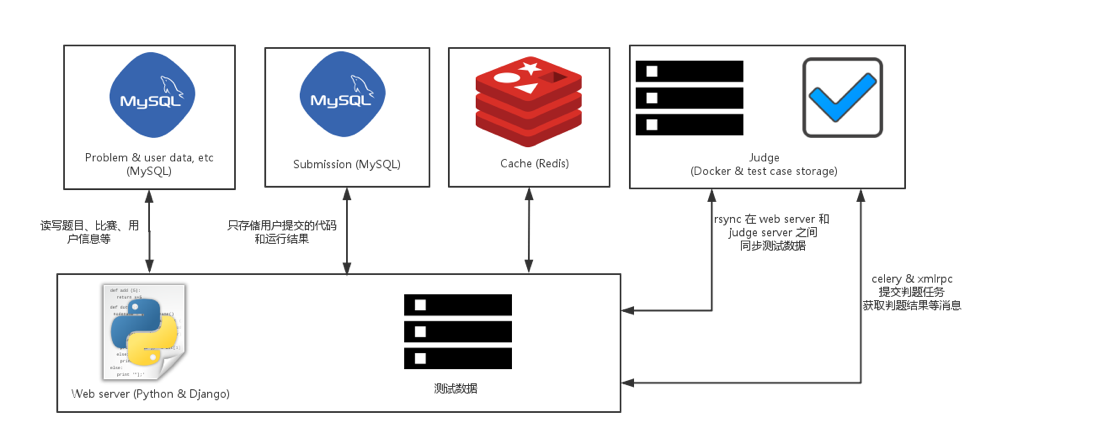
\includegraphics[width=0.9\textwidth]{oj-structures}
\caption{OJ后端架构图}
\end{figure}

Web前端使用了Bootstrap作为前端UI框架,使用了avalon作为 MVVM框架。由于JavaScript数量非常多,依赖关系也很复杂,所以还使用了require.js进行JavaScript模块化,使用了r.js进行静态文件的压缩和合并。

\subsection{功能模块}

\begin{figure}[H]
\centering
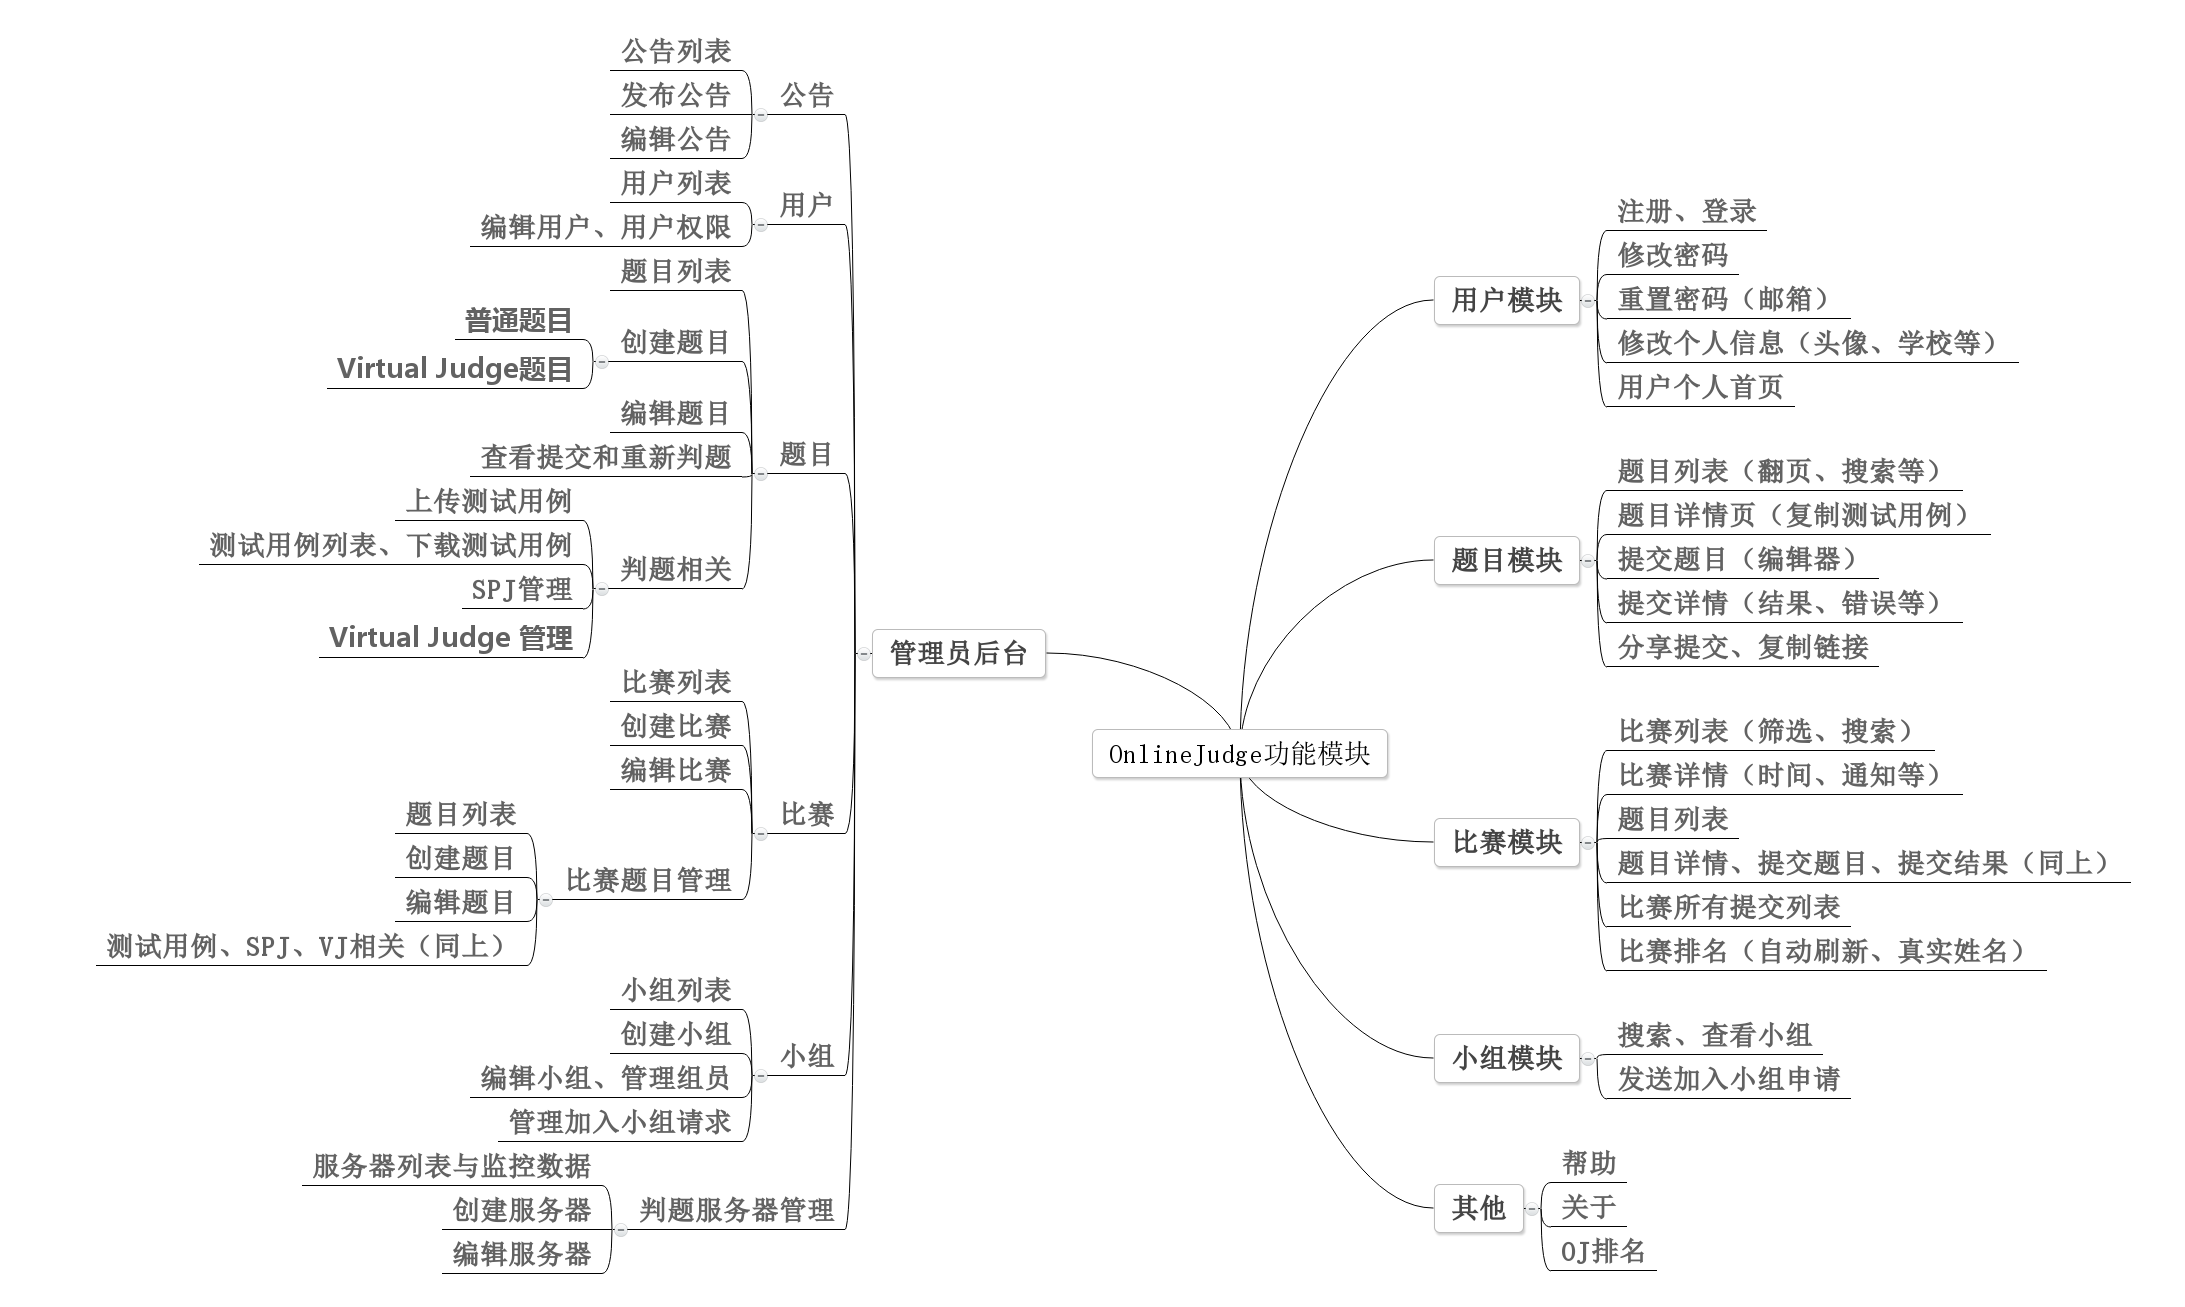
\includegraphics[width=\textwidth]{OJ-module}
\caption{OJ功能模块}
\end{figure}


\clearpage
\section{Web后端实现}

OJ的后端是基于Python和Django的,数据库使用MySQL,缓存及队列使用Redis和Celery。

\subsection{Django框架模块组成}

\subsubsection{Model数据库模型}
Model是数据模型,是Django ORM的重要组成部分。使用ORM可以大大简化数据库操作,提高开发效率,同时避免SQL注入等安全问题的发生。一般情况下一个Model映射到数据库中的一张表中,Model的每一个属性就是表中的每一个字段。比如说

\begin{verbatim}
class User(models.Model):
    username = models.CharField(max_length=64, unique=True, db_index=True)
    # 真实姓名
    real_name = models.CharField(max_length=30, blank=True, null=True)
    password = models.CharField(max_length=128)
    # 0是普通用户,管理员为1,超级管理员为2
    admin_type = models.IntegerField(default=0)
    email = models.EmailField(max_length=256, blank=True, null=True)
\end{verbatim}就会生成如下所示创建表的SQL语句。

\begin{verbatim}
CREATE TABLE user(
    id INT PRIMARY KEY,
    username VARCHAR(64) UNIQUE NOT NULL,
    real_name VARCHAR(30),
    password VARCHAR(128) NOT NULL,
    admin_type INT NOT NULL,
    email VARCHAR(256)
)
\end{verbatim}
如果需要创建用户名为foo的用户,可以使用\\\texttt{User.objects.create(username="foo", password="hidden", email="foo@gmail.com")}。如果需要查询用户名foo的用户,可以使用\texttt{user = User.objects.get(username="foo")},Django就会自动的将其转换为SQL语句\texttt{SELECT id, username, password, email FROM user WHERE username="foo";},然后就可以访问\texttt{user}对象的属性来获取具体字段的值。

如果需要修改用户信息,可以直接给属性赋值,然后调用\texttt{saeve}方法即可。比如
\begin{verbatim}
user.emai="foo@example.com"
user.save()
\end{verbatim}Django就可以生成对应的SQL update语句。

\subsubsection{View视图处理函数}

View视图处理函数就是业务逻辑所在了,负责处理各种请求、进行数据校验、与数据库进行交互和调用第三方API等。

Django的View处理函数都是与URL绑定的,符合该URL规则的请求就会进入对应的View函数处理。比如

\begin{verbatim}
url(r'^problem/(?P<problem_id>\d+)/$', "problem.views.problem_page")

def problem_page(request, problem_id):
    try:
        problem = Problem.objects.get(id=problem_id, visible=True)
    except Problem.DoesNotExist:
        return error_page(request, u"题目不存在")
    return render(request, "oj/problem/problem.html", {"problem": problem})
\end{verbatim}

View视图处理函数一般接收\texttt{request}和部分URL中匹配的值为参数,需要返回一个\texttt{HTTPResponse}对象。

\subsection{部分模块功能实现}
下面将以部分逻辑比较复杂的模块为例,详细分析OJ后端的开发过程。

\subsubsection{用户登录}
用户登录是几乎所有网站必备的基础功能。用户提交用户名和密码,然后数据POST到后端进行查询和验证,如果验证通过,就设置Cookies,否则提示用户名或密码错误。

\begin{verbatim}
class UserLoginAPIView(APIView):
    def post(self, request):
        """
        用户登录json api接口
        ---
        request_serializer: UserLoginSerializer
        """
        serializer = UserLoginSerializer(data=request.data)
        if serializer.is_valid():
            data = serializer.data
            user = auth.authenticate(username=data["username"], password=data["password"])
            # 用户名或密码错误的话 返回None
            if user:
                auth.login(request, user)
                return success_response(u"登录成功")
            else:
                return error_response(u"用户名或密码错误")
        else:
            return serializer_invalid_response(serializer)
\end{verbatim}

这里使用了Django Rest Framework的\texttt{APIView},可以简化通过AJAX和API通信的Web程序的开发,这里只实现了\texttt{POST}函数,如果不是\texttt{POST}方法请求API就会收到错误响应。

\texttt{serializer}是用来校验数据的,写法和Model类似,需要规定字段和对应的数据类型等,\texttt{UserLoginSerializer}的实现代码是

\begin{verbatim}
class UserLoginSerializer(serializers.Serializer):
    username = serializers.CharField(max_length=64)
    password = serializers.CharField(max_length=128)
\end{verbatim}

如果缺少字段或者字段的数据不符合要求,就会返回一个\\\texttt{serializer\_invalid\_response(serializer)}的响应,这是一个封装后的函数,实现代码是

\begin{verbatim}
def serializer_invalid_response(serializer):
    for k, v in serializer.errors.iteritems():
        return error_response(k + " : " + v[0])
\end{verbatim}

通过\texttt{serializer.errors}属性可以得到错误详情,然后返回前端,提示用户。

如果数据校验通过,就会使用用户名和密码作为参数,调用Django的\texttt{auth.authenticate}方法进行验证。\texttt{auth.authenticate}实现也比较简单,首先根据配置文件选择密码的哈希函数计算密码的哈希值,然后使用用户名和哈希值去数据库查询,如果查询到记录,说明用户名密码正确,返回对应的\texttt{User}对象。

因为HTTP协议是一个无状态的协议,服务器端需要通过Cookies来将请求和登录的用户进行对应,这个对应关系是保存在服务器端的,有时也称为\texttt{Session},这个过程就是\texttt{auth.login(request, user)}实现的。

Django生成的数据库中有\texttt{django\_session}表,表中有三个字段,\texttt{session\_key}、\texttt{session\_data}和\texttt{expire\_date}。首先Django会在这张表中插入一条记录,简化的demo如下。

\begin{verbatim}
DjangoSession.objects.create(session_key=random_string(), 
                             session_data=json.dumps({"user_id": user.id}), 
                             expire_date=some_date())
\end{verbatim}

然后使用\texttt{set-cookie} HTTP头给浏览器设置一个Cookie,比如\texttt{set-cookie:sessionid=\\9400de64wpdhtd8w5s82ntvy6ht3nsd5; expires=Wed, 18-May-2016 13:13:34 GMT; httponly; Max-Age=1209600; Path=/},key是\texttt{sessionid},value是数据库里的\texttt{session\_key},还包括过期时间等信息。

这样每次用户请求的时候,取到Cookies中\texttt{sessionid}的值,再去表中查询就可以得到当前用户的ID了。

\subsubsection{重置密码}

重置密码功能的设计关乎用户用户账户的安全,已经有很多案例说明重置密码功能设计缺陷带来的安全问题\cite{password-reset-vul}。

用户提交重置密码请求后,首先会查询邮箱是否存在,如果存在,就会生成32位长度的随机token和30分钟的过期时间。然后调用异步队列,向该邮箱发送重置密码链接,响应前端重置邮件已发出。

用户收到邮件之后,点击重置链接,后端会先验证该链接的有效性,包括是否存在和是否过期,如果验证通过就会返回重置密码页面。用户填写新密码提交后,会再次验证token的有效性,如果验证通过,就会查询该token对应的用户,然后更新密码。

\begin{figure}[H]
\centering
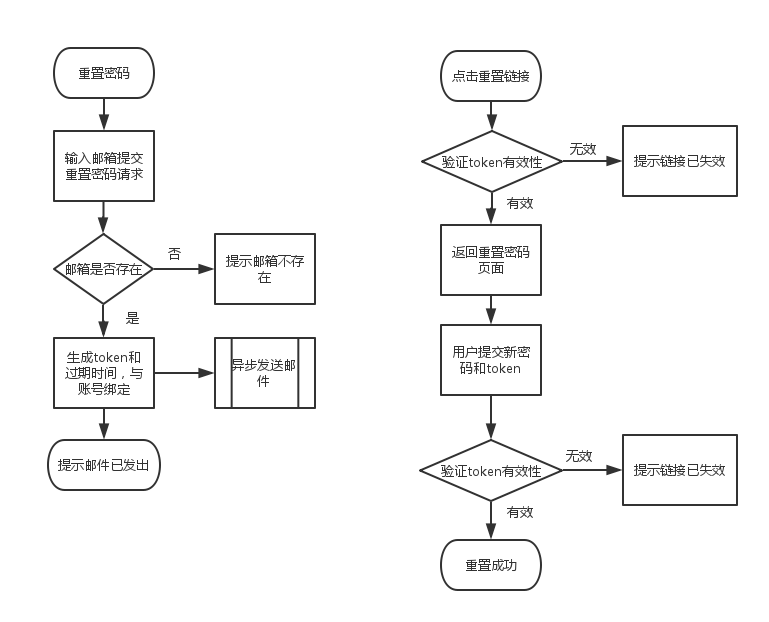
\includegraphics[width=0.6\textwidth]{password-reset-flow}
\caption{密码重置流程}
\end{figure}

\subsubsection{比赛排名}
比赛排名的Model是
\begin{verbatim}
class ContestRank(models.Model):
    user = models.ForeignKey(User)
    contest = models.ForeignKey(Contest)
    total_submission_number = models.IntegerField(default=0)
    total_ac_number = models.IntegerField(default=0)
    total_time = models.IntegerField(default=0)
    submission_info = JSONField(default={})
\end{verbatim}

可以看到,记录了具体题目提交信息的字段保存的是JSON数据,格式是\texttt{\{\$problem\_id: \{"is\_ac": True/False, "ac\_time": \$ac\_time, "error\_number":\$error\_number, \\"is\_first\_ac": True/False\}\}}这样可以简化数据库设计的难度,让SQL数据库按照NoSQL来用。这样每一个用户就是一条记录,也就是排名上的一行。只要根据\texttt{contest\_id}查询一次数据库后,就可以得到生成页面的全部数据。

鉴于比赛参与人数可能很多,排名数据偏大,如果每次重新生成,可能会遇到性能问题,我们在这里使用了Redis作为缓存,在HUSTOJ等系统中也有类似的用法\cite{hustoj-cache}。使用\texttt{\$\{contest\_id\}\_rank\_cache}作为缓存的key。每次生成页面的时候,先使用缓存key去Redis中取数据,如果没有取到,就去MySQL中查询,同时生成Redis缓存。每次有新的提交的时候,异步队列需要主动的清除Redis缓存,避免页面数据过期。
\subsection{判题模块}

\subsubsection{选择判题服务器}
在OJ使用人数较多的情况下,需要使用多台服务器进行判题。选择哪一台服务器,怎么均衡服务器负载,怎么与服务器通信、怎么得到服务器判题结果就是我们要面对的问题了。

管理员可以在admin后台配置多台判题服务器,每台服务器都有自己的最大判题实例数量\texttt{max\_instance\_number}、当前使用的判题实例数量\texttt{used\_instance\_number}和负载\texttt{workload}三个指标,每次分配给该服务器一个判题任务,当前已经使用的实例数加一,服务器的负载workload就会修改为${\frac {used\_instance\_number}{max\_instance\_number}} \times 100$ \%,判题结束的时候,当前已经使用的实例数减一,负载值也对应修改。分配给该服务器同时运行的任务不会超过该服务器的最大判题实例的值。

\subsubsection{RPC通信}
XML-RPC是一个远程过程调用(remote procedure call,RPC)的分布式计算协议,通过XML将调用远程机器上的函数封装,一般使用HTTP协议作为通信协议。

在远程机器上启动XML-RPC Server,注册\texttt{JudgeInstanceRunner}类,供远程调用。

\begin{verbatim}
server = AsyncXMLRPCServer(('0.0.0.0', 8080), SimpleXMLRPCRequestHandler)
server.register_instance(JudgeInstanceRunner())
server.serve_forever()
\end{verbatim}

由上一部分选择好服务器后,指定服务器的IP和端口就可以运行代码了。

\begin{verbatim}
s = TimeoutServerProxy("http://" + judge_server.ip + 
                             ":" + str(judge_server.port), timeout=30)
data = s.run(judge_server.token, self.submission.id, self.submission.language,
             self.submission.code, self.time_limit, self.memory_limit, 
             self.test_case_id, self.spj, self.spj_language,
             self.spj_code, self.spj_version)
\end{verbatim}

\subsubsection{用户代码的运行过程}
在判题服务器上,有对应语言的编译参数和运行参数配置。以下是C语言的编译和运行参数。

\begin{verbatim}
{
    "name": "c",
    "src_name": "main.c",
    "code": 1,
    "compile_max_cpu_time": 3000,
    "compile_max_memory": 128 * 1024 * 1024,
    "compile_command": "/usr/bin/gcc -DONLINE_JUDGE -O2 \
                        -w -fmax-errors=3 -std=c99 {src_path} -lm -o {exe_path}/main",
    "spj_compile_command": "/usr/bin/gcc -DONLINE_JUDGE -O2 \
                            -Werror -fmax-errors=3 -std=c99 {src_path} -lm -o {exe_path}",
    "execute_command": "{exe_path}/main",
    "use_sandbox": True
}
\end{verbatim}

首先按照参数编译用户代码,可执行文件存放在指定的目录。如果出现编译错误或者编译器异常,直接返回错误信息,提示编译错误。如果编译通过,将会在沙箱中运行用户代码,\texttt{stdin}的输入来自于上传的测试用例文件重定向,进程的\texttt{stdout}会重定向到指定的输出文件。

进程正常结束后,系统将会计算重定向输出文件去除最后的空格和换行后的md5,与上传的测试用例的md5(这些数据已经保存在文件的meta信息中了)进行比较,如果一致,说明测试通过,否则是答案错误。

如果进程非正常结束,会返回运行错误等信息。这些细节将在后文判题沙箱中详述。

如果这个提交对应的题目是Special Judge类型,那上面的判断过程是由出题人上传的代码来执行的。每个Special Judge都有一个版本号,每次更新后会变。如果发现目录中没有当前版本号的SPJ程序,系统就会先编译SPJ的代码,这样就解决了更新SPJ代码后无法重新编译的问题。

SPJ代码需要按照一定的模板来写,测试用例文件和用户输出文件的路径将会作为两个参数传递给Special Judge,然后通过进程返回值来获取判题结果。

\subsubsection{判题结束后的各种动作}

服务器判题结束后,还有一系列的动作需要执行,包括:

\begin{itemize}
    \item[-] 更新题目提交数量和AC数量计数器
    \item[-] 更新用户做题状态计数器,用于题目前面显示对应的符号
    \item[-] 更新用户做题数量和AC数量计数器
    \item[-] 比赛排名缓存的刷新
\end{itemize}

\subsection{Virtual Judge的实现}

\subsubsection{简介}

Virtual Judge是一种特殊的OJ系统。与其他OJ系统不同的是,Virtual Judge系统本身并没有任何测试数据,而是通过在其他OJ系统中的机器人账号进行测试并抓取测试结果。因此可以在只有题目而没有测试数据的前提下建立竞赛。\cite{wiki-vj}

\subsubsection{插件式爬虫}

对于每个OJ,具体的处理方法和过程都是不同的,但是最终要实现的功能都是统一的,比如登录用户、获取指定URL的题目、提交题目和获取指定的提交结果。在这种情况下,我们可以让每个OJ的爬虫都继承一个父类,需要实现父类中所有的公开方法,如果子类没有实现该方法,调用的时候就会引发\texttt{NotImplementedError}异常。

\begin{figure}[H]
\centering
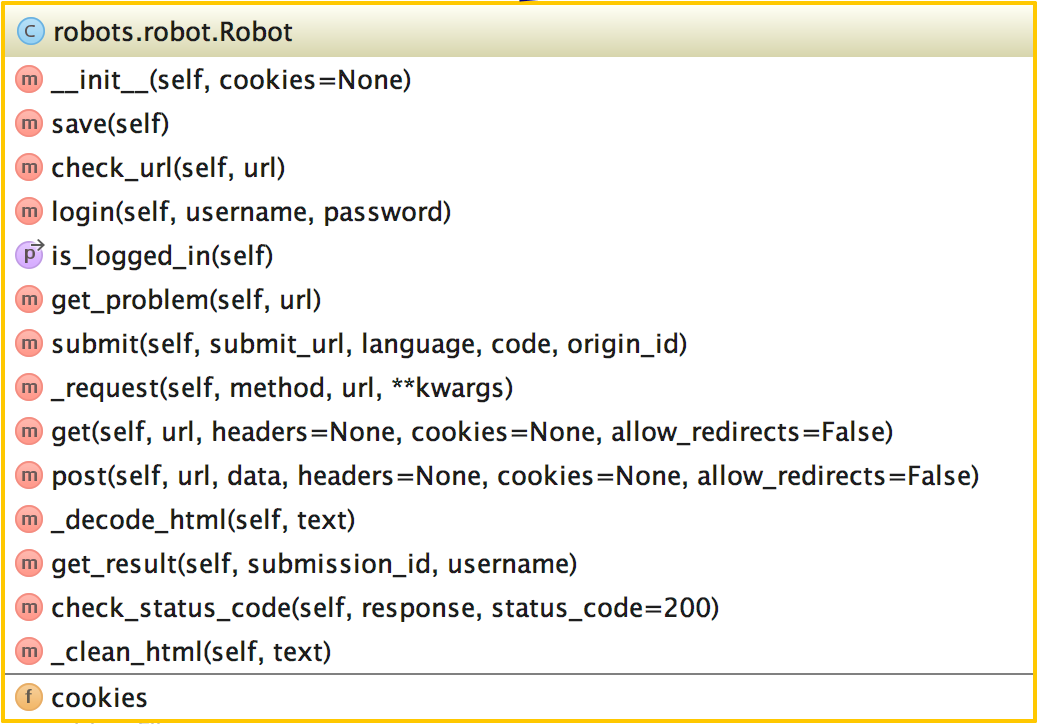
\includegraphics[width=0.6\textwidth]{robot-uml}
\caption{爬虫父类的UML}
\end{figure}

部分函数的作用:
\begin{itemize}
    \item[-] \texttt{save}:返回登陆后Cookies和token信息
    \item[-] \texttt{check\_url}:检查是否是本OJ题目的URL
    \item[-] \texttt{login}:使用给定的用户名密码登录OJ
    \item[-] \texttt{get\_problem}:获取指定URL的题目信息
    \item[-] \texttt{submit}:提交题目
    \item[-] \texttt{get}和\texttt{post}:HTTP协议请求网络
    \item[-] \texttt{get\_result}:获取提交结果
\end{itemize}

\subsubsection{工作流程}

以获取杭州电子科技大学OJ题目详情为例,具体实现的逻辑是:

\begin{verbatim}
def get_problem(self, url):
    if not self.check_url(url):
        raise RequestFailed("Invaild Hduoj url")
    regex = {"title": r"<h1 style='color:#1A5CC8'>(.*)</h1>",
             "time_limit": r"Time Limit:\s*[\d]*/([\d]*)\s*MS",
             "memory_limit": r"Memory Limit:\s*[\d]*/([\d]*)\s*K",
             "description": r"Problem Description</div>\s*
                              <div class=panel_content>([\s\S]*?)</div>",
             "input_description": r"Input</div>\s*
                                    <div class=panel_content>([\s\S]*?)</div>",
             "output_description": r"Output</div>\s*
                                     <div class=panel_content>([\s\S]*?)</div>",
             "hint": r"Hint(?:[\s\S]*?Hint[\s\S]*?</i>|
                       </i>\s*</div>)([\s\S]*?)</div>",
             "spj": r"<font color=red>Special Judge</font>",
             "samples": r'Courier New,Courier,monospace;">([\s\S]*?)(?:<div|</div>)'}
    problem_id = re.compile(r"\d{4}").search(url).group()
    data = self._regex_page(url, regex)
    data["id"] = problem_id
    data["submit_url"] = "http://acm.hdu.edu.cn/submit.php?action=submit"
    return data
\end{verbatim}

以提交题目并获取提交结果为例,分析爬虫提交题目的的工作逻辑。此步骤涉及到多个异步任务。

首先根据请求数据中的题目id获取给题目对应的OJ的具体信息,在VJ数据库中创建该提交的记录,查询当前是否有空闲的爬虫用户用于提交。

如果没有空闲的爬虫用户,该提交就会被放入一个等待队列中,返回提交信息,否则将会修改该用户的标志位,设置为被占用。

然后会根据OJ的设置和该用户的登录信息实例化一个对应的爬虫,传递所需参数,创建\texttt{submit\_dispatcher}异步任务,得到\texttt{task\_id},更新到数据库,返回调用者提交信息。这时,爬虫在后端异步的运行。

而\texttt{submit\_dispatcher}异步任务会去创建真正的提交异步任务\texttt{submit},同时还会设置该异步任务的回调函数为\texttt{submit\_waiting\_submission}和\texttt{update\_submission},然后将该\texttt{task\_id}更新到数据库中。

\texttt{submit}方法会调用爬虫的\texttt{submit}方法去提交代码,接着循环请求判题结果,直到得到结果或者超过最多尝试次数,最终返回结果。

等到\texttt{submit}执行完毕的时候,两个回调函数会被调用,功能分别是提交等待队列中的题目和更新该次提交的信息。如果等待队列中没有提交,就会释放该爬虫用户,否则直接使用该用户继续提交题目,回到本流程开头。

\subsection{安全问题}

\subsubsection{用户密码存储}

现代网站已经不再使用明文密码存储的方式了,而是改用只在数据库中存储明文密码的哈希。常见的哈希算法有MD5和SHA,可以从任何一段字符串计算出一段固定长度的哈希值。这样当用户输入密码时,直接将该密码代入算法得出哈希值,再与存储的哈希值对比,相同则允许登录。用户注册时也是直接存储密码的哈希值,而不是明文密码。这样就防止数据库泄露的时候导致用户明文密码泄露。

但是随着计算能力大幅提高,MD5和SHA1算法已经不再推荐使用了,这些算法被碰撞的几率已经越来越大了。本系统中存储密码使用的Django默认哈希方法,SHA256加salt后使用PBKDF2算法处理,该算法计算消耗的CPU时间非常多,能大大减慢暴力破解速度。

\subsubsection{XSS}

XSS漏洞跨站脚本攻击,是Web程序中常见的漏洞。其原理是攻击者向有XSS漏洞的网站中传入恶意的HTML和JavaScript代码,当其它用户浏览该网站时,JavaScript代码会自动执行,从而达到攻击的目的。比如盗取用户Cookie、重定向到其它网站等。

Django模板默认对模板输出全部转义,避免了绝大多数的XSS问题。但是有一些输出是不能转义的,比如公告的内容、题目的说明等,它们是使用富文本编辑器进行编辑的,如果进行过滤,文字的样式就无法显示了。所以我们在这里需要过滤危险的JavaScript和HTML属性等,使用了https://github.com/phith0n/python-xss-filter作为过滤器。

\subsubsection{SQL注入}

SQL注入攻击,是Web开发中最常见的一种安全漏洞。可以用它来从数据库获取敏感信息,甚至有可能获取数据库乃至系统用户最高权限。而造成SQL注入的原因是因为程序没有有效过滤用户的输入,使攻击者成功的向服务器提交恶意的SQL查询代码,程序在接收后错误的将攻击者的输入作为查询语句的一部分执行,导致原始的查询逻辑被改变,额外的执行了攻击者的代码。

OJ系统全部使用Django的ORM进行数据库查询,而ORM在进行查询的时候使用了SQL参数绑定,所以不存在SQL注入的风险。

\subsubsection{CSRF}

CSRF可以伪造受信任用户的请求来利用受信任的网站。攻击者可以在第三方网站hacker.com设置代码,用户在浏览这些网页的时候向victim.com跨域发送数据,浏览器根据同源策略,带上了victim.com的cookies,导致请求被伪造,可能造成很大的危害,比如发送微博、添加管理员、修改密码等。

OJ系统采取的措施是需要修改服务器状态的请求全部增加token验证,token是在Cookies中读取的,而根据同源策略,hacker.com是无法读取victim.com的Cookies的,这样就无法伪造token。后端服务器只要对比Cookies中的token和请求头中的token是否一致就可以了。

\subsubsection{沙箱安全}

沙箱安全是整体开发中的重点和难点,本文将在第5章中详细分析。
     
\subsubsection{其他安全问题}

上面提到的几个安全问题是出现频率比较高的,危害比较大的。还有一些其他的安全问题没有单独列出,比如密码暴力破解、恶意提交请求等。

针对密码暴力破解,增加了管理员密码的两步验证。管理员在登录的时候,必须同时输入手机动态密码app上显示的验证码。针对恶意注册,增加了验证码。

针对使用脚本进行大量恶意提交的问题,使用Token Bucket机制增加了频率限制,同时为一定的并发请求预留了空间。当用户触发频率限制的时候,将会得到提交失败的提示和需要等待的时间。

\clearpage
\section{Web前端实现}

OJ系统中前端页面主要分为两部分,用户前台和admin后台,两部分应用场景有着明显的差异。用户前台,逻辑简单,主要以展示为主,需要兼顾搜索引擎的抓取;admin后台,界面逻辑非常复杂,有大量的列表页、动态验证项目、动态变化的表单,不需要考虑搜索引擎的抓取问题。需要进行实际的分析,选择不同的开发技术。

\subsection{admin后台的SPA页面实现}

\subsubsection{JavaScript模块化}

页面功能的复杂化往往伴随的是JavaScript代码的数量的爆炸,传统的使用\texttt{script}标签直接加载的方案会遇到很多问题,比如无法确定模块依赖顺序、文件合并复杂等。由于历史原因,JavaScript 并未提供一种原生的、语言级别的模块化组织模式,而是将模块化的方法交由开发者来实现。因此,出现了很多种 JavaScript 模块化的实现方式,比如,CommonJS Modules、AMD 等。我们使用了AMD的模块化方案,由require.js充当加载器\cite{js-module}。

\begin{verbatim}
define("bsAlert", ["jquery", "bootstrap"], function($){
     function bsAlert(content){
         // TODO
     }
    return bsAlert;
});
\end{verbatim}

\texttt{bsAlert}是模块名,\texttt{jquery}和\texttt{bootstrap}是模块的依赖,加载\texttt{bsAlert}模块的时候,require.js会自动去加载它的依赖模块。

使用\texttt{require}函数引用这个模块,获得函数引用。

\begin{verbatim}
require(["bsAlert"], function (bsAlert) {
    bsAlert("foobar");
})
\end{verbatim}

同时,由于已经确定模块间依赖关系,r.js可以将模块级别和页面级别的JavaScript合并成一个文件,这样就减少了页面上的网络请求次数,提高了性能和用户体验。以admin后台添加题目为例:

\begin{table}[H]
\centering  % 表居中
\caption{合并JavaScript前后网络请求统计}
\begin{tabular}{|c|c|c|}  % {lccc} 表示各列元素对齐方式,left-l,right-r,center-c
\hline
是否合并 &网络请求次数 &网络请求数据量\\ \hline  % \hline 在此行下面画一横线
否 &43 &1.3M\\         % \\ 表示重新开始一行
\hline
是 &15 &844K\\
\hline
\end{tabular}
\end{table}

\subsubsection{MVVM框架}

在传统前端开发中,大量的动态效果需要直接进行DOM操作和拼接HTML操作,这是造成JavaScript代码无法维护的元凶之一,使用MVVM框架可以不再手动操作DOM,简化了操作,而且可以提高性能。OJ系统使用的是avalon.js框架,类似的框架还有 Vue.js和Angular JS。

所有前端代码彻底分成两部分,视图的处理通过绑定实现,业务逻辑则集中在VM对象中处理。我们只要操作VM的数据,它就自动的同步到视图。demo如下:

\begin{verbatim}
<script>
var vm = avalon.define({
    $id: "demo",
    name: "foobar"
})
</script>

<body ms-controller="demo">
    <input ms-duplex="name">
    <p>Hello,{{name}}!</p>
</body>
\end{verbatim}

这样页面加载的时候,文本框和"hello"后面中就会显示"foobar",然后随着用户修改文本框中的文字,页面上"hello"后面的文字也会自动改变。

\subsubsection{Web组件}
前端开发的时候经常会遇到一些重复的功能和逻辑,比如翻页模块、上传模块、富文本编辑器等,将底层的UI组件与自己的业务逻辑联系在一起然后复用才能提高开发效率,增强代码的可维护性。admin后台有多个封装的Web组件,以翻页pager组件为例。

\begin{verbatim}
avalon.component("ms:pager", {
    $template: "页数: {{ currentPage }}/{{ totalPage }} " +
    "<button ms-class=\"{{ currentPage==1?'btn disabled':'btn' }}
    \"ms-click=\"_getPrevPage\">上一页</button> " +
    " <button ms-class=\"{{ currentPage==totalPage?'btn disabled':'btn' }}
    \" ms-click=\"_getNextPage\">下一页</button>",
    currentPage: 1,
    totalPage: 1,
    _getPrevPage: _interface,
    _getNextPage: _interface,
    $init: function (vm, el) {
        vm._getPrevPage = function () {
            if (vm.currentPage > 1) {
                vm.currentPage--;
                vm.getPage(vm.currentPage);
            }
        };
        vm._getNextPage = function () {
            if (vm.currentPage < vm.totalPage) {
                vm.currentPage++;
                vm.getPage(vm.currentPage);
            }
        };
    }
\end{verbatim}

在页面上只要使用
\begin{verbatim}
<ms:pager $id="userPager" config="pager"></ms:pager>
\end{verbatim}就可以得到有完整功能的翻页按钮,不需要每个页面都去重复代码,而且不需要关心内部实现。

\subsubsection{前后端分离}

我们在传统前端开发过程中有很多痛点:

\begin{itemize}
\item[-] 前端开发依赖后端,一般需要后端功能完成后,由后端向前端模板传递变量完成渲染,才能进行开发和测试,而且前端可能需要搭建后端开发环境。或者前端先完成一个demo页面,然后由后端工程师转换为实际的框架模板。
\item[-] 前端模板中有大量的后端语言逻辑,导致模板维护性变差。
\item[-] 前端模板数据更新需要刷新页面,而整个页面的完全加载是对带宽和性能的浪费。
\end{itemize}

由于网页前端越来越复杂,为了提升开发和测试效率,前后端分离的技术使用的越来越多,后端主要负责业务逻辑实现和提供API接口,前端负责构建页面和展示数据。

\subsubsection{admin后台整体框架}
由于admin后台是一个SPA页面,页面无刷新,URL不会变化,所以需要使用URL中的hash存储页面路由信息。比如\texttt{/admin/\#announcement/announcement}、\texttt{/admin/\#user/user\_list}等,JavaScript监听hash变化事件,修改\texttt{vm.templateUrl},加载不同的HTML模板。

\begin{verbatim}
<div ms-include-src="templateUrl" data-include-replace="true"></div>
\end{verbatim}

\begin{figure}[H]
\centering
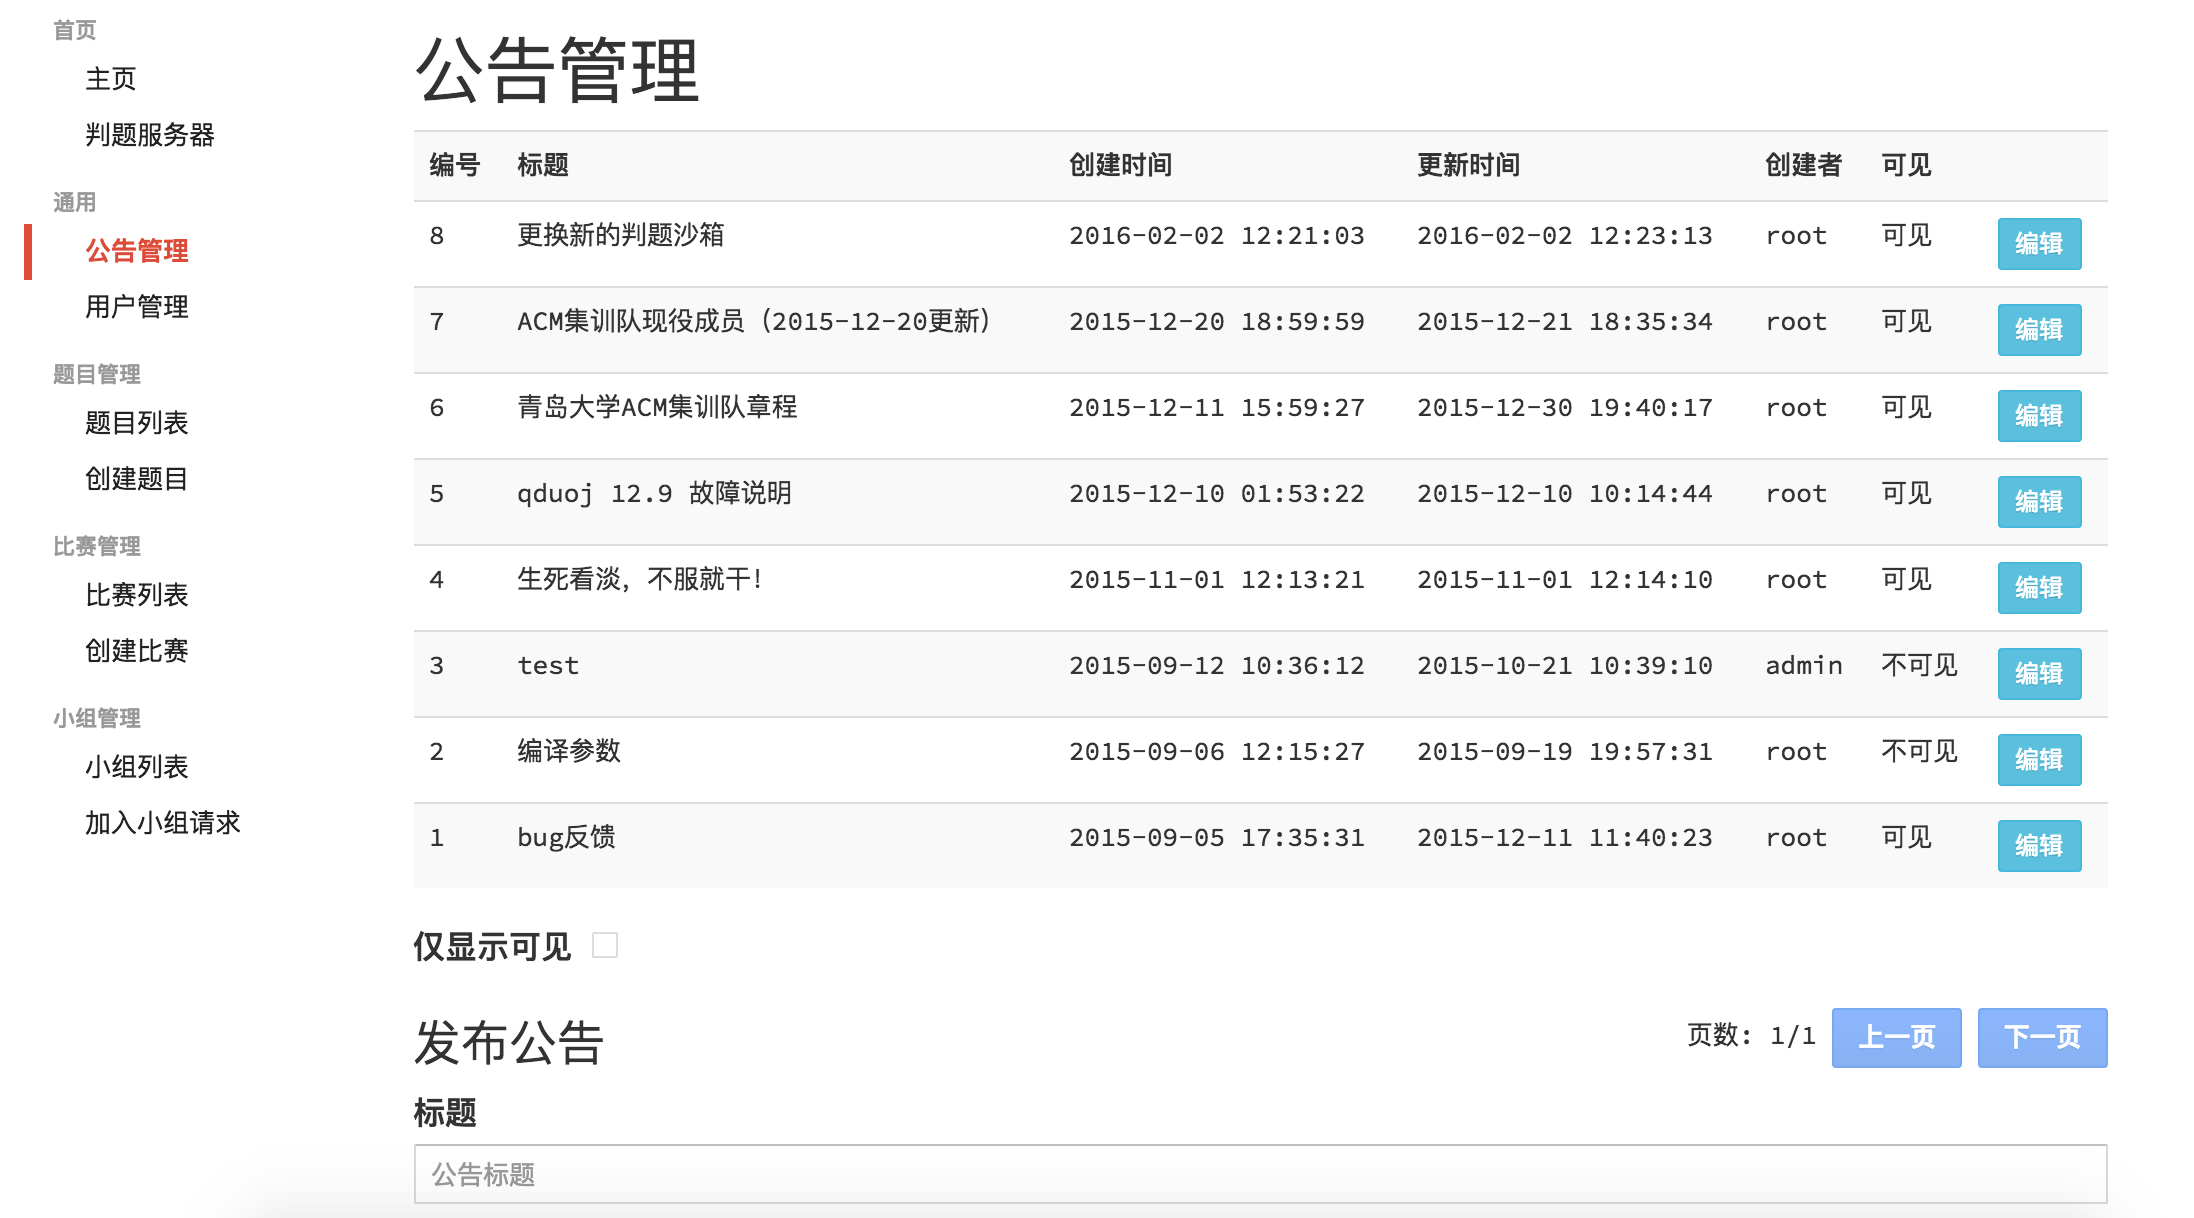
\includegraphics[width=0.9\textwidth]{admin-index}
\caption{admin首页}
\end{figure}

\subsubsection{用户管理页面的实现}
本节将以后台用户管理页面为例,解释admin模块前端开发的流程。

用户管理页面主要分为用户翻页列表和用户编辑两部分。对于用户列表,在VM中存储一个数组,然后在前端模板进行循环。

\begin{verbatim}
var vm = avalon.define({
    $id: "userList",
    userList: []
}
\end{verbatim}

HTML模板的部分代码

\begin{verbatim}
<tr ms-repeat="userList">
    <td>{{ el.id }}</td>
    <td>{{ el.username }}</td>
    <td>{{ el.create_time|date("yyyy-MM-dd HH:mm:ss")}}</td>
    <td>{{ el.real_name }}</td>
    <td>{{ el.email }}</td>
</tr>
\end{verbatim}

页面加载的时候,JavaScript通过ajax去后端查询分页用户列表,然后赋值给vm.userList,这时HTML模板中就会自动显示为列表项目。

\begin{verbatim}
function getPage(page) {
    var url = "/api/admin/user/?paging=true&page=" + page + "&page_size=10";
    $.ajax({
        beforeSend: csrfTokenHeader,
        url: url,
        dataType: "json",
        method: "get",
        success: function (data) {
            if (!data.code) {
                vm.userList = data.data.results;
                avalon.vmodels.userPager.totalPage = data.data.total_page;
            }
            else {
                bsAlert(data.data);
            }
        }
    });
}
\end{verbatim}

\begin{figure}[H]
\centering
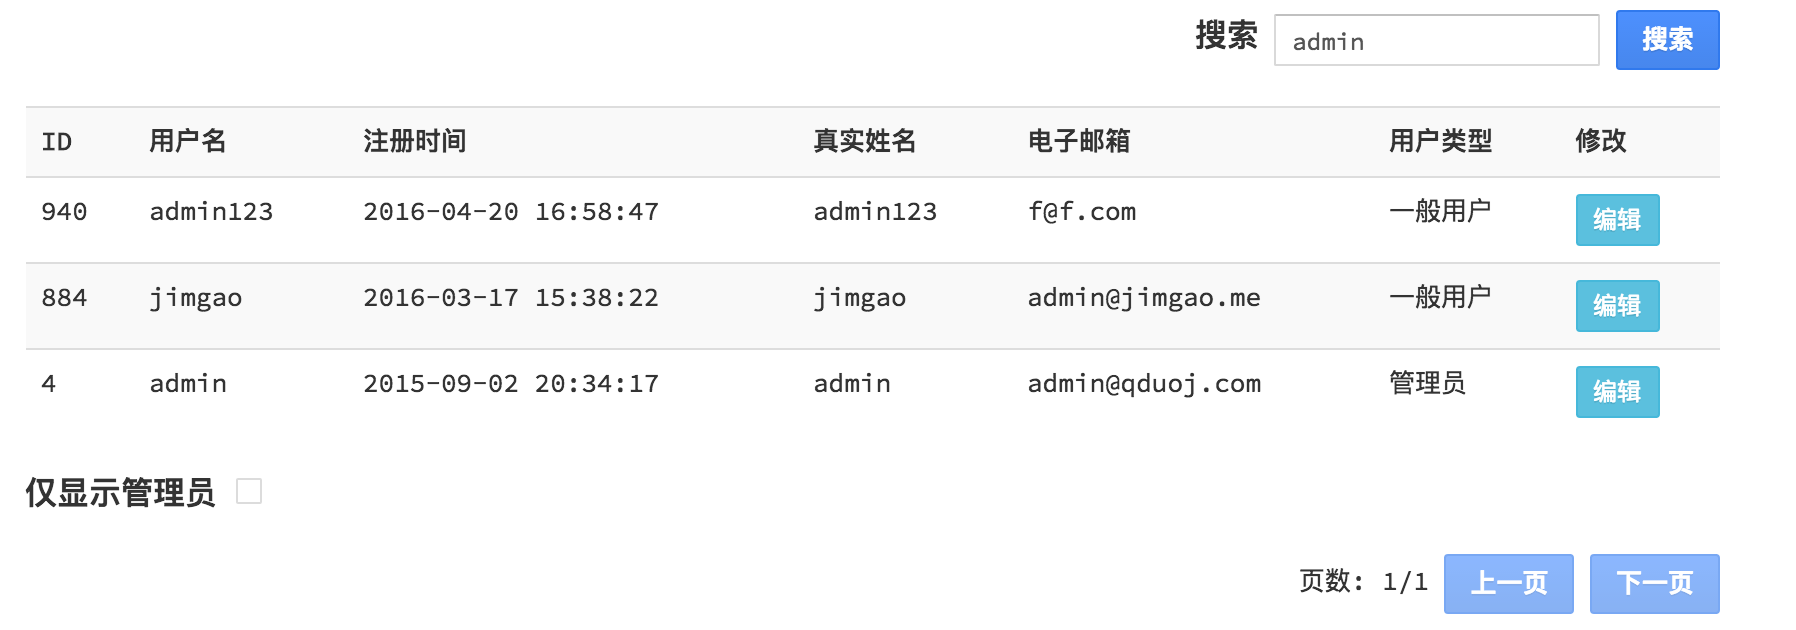
\includegraphics[width=0.9\textwidth]{admin-users}
\caption{admin用户列表}
\end{figure}

编辑用户的时候,需要VM中增加几个同步变量,比如\texttt{name}、\texttt{email}等,然后与input双向绑定。以用户名为例。

\begin{verbatim}
<div class="form-group col-md-4"><label>用户名</label>
    <input type="text" class="form-control" ms-duplex="username"
           data-minlength="3" data-minlength-error="用户名不得少于3位" required>
    <div class="help-block with-errors"></div>
</div>
\end{verbatim}

vm.username的修改将导致页面显示的修改,用户输入用户名将导致vm.username的修改。

最后通过AJAX请求后端更新用户信息

\begin{verbatim}
$("#edit-user-form").validator()
.on('submit', function (e) {
    if (!e.isDefaultPrevented()) {
        var data = {
            username: vm.username,
            email: vm.email,
            // 省略部分属性
        };
        $.ajax({
            url: "/api/admin/user/",
            data: data,
            dataType: "json",
            method: "put",
            success: function (data) {
                if (!data.code) {
                    bsAlert("编辑成功!");
                    getPage(1);
                } else {
                    bsAlert(data.data);
                }
            }
        });
        return false;
    }
});
\end{verbatim}

\begin{figure}[H]
\centering
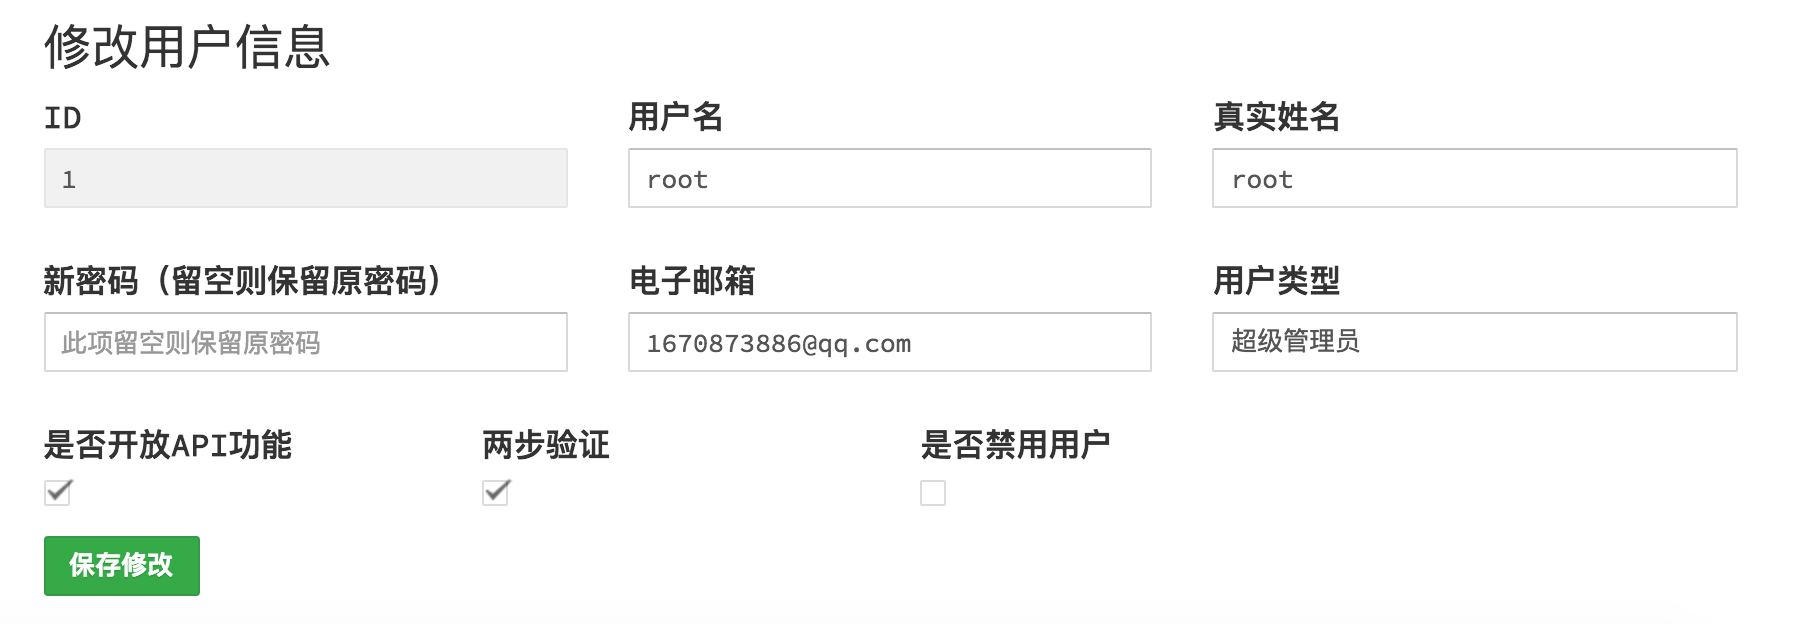
\includegraphics[width=0.9\textwidth]{admin-edit-user}
\caption{admin编辑用户}
\end{figure}

在更加复杂的页面上也是类似的思路,只是使用了更多的绑定、Web组件和更加复杂的业务逻辑和动态效果。

\subsection{用户前台的后端渲染页面}

和前后端分离然后前端渲染页面相比较,后端渲染要简单的多,也是最传统的做法。因为Django是MVC的架构,我们View中的逻辑去Model中查询,然后传递给模板就可以了。模板中变量占位符将渲染为实际的值,还可以使用简单的逻辑判断,还可以调用函数。

以题目详情页为例:

\begin{verbatim}
def problem_page(request, problem_id):
    try:
        problem = Problem.objects.get(id=problem_id, visible=True)
    except Problem.DoesNotExist:
        return error_page(request, u"题目不存在")
    return render(request, "oj/problem/problem.html", {"problem": problem})
\end{verbatim}

部分模板的代码

\begin{verbatim}
<div class="problem-section">
    <label class="problem-label">描述</label>
    <div class="problem-detail">{{ problem.description|safe }}</div>
</div>
<div class="problem-section">
    <label class="problem-label">输入</label>
    <p class="problem-detail">{{ problem.input_description }}</p>
</div>
\end{verbatim}
\clearpage
\section{判题沙箱的设计}
\subsection{总体分析}
判题沙箱是保证OJ系统安全的重要措施之一,如果没有沙箱,直接在服务器上运行用户的代码是存在严重安全风险\cite{wooyun-oj-vul}的,而且也无法去控制或获取代码的运行时间、占用内存大小和运行结果等运行数据。

沙箱要实现的功能:

\begin{itemize}
\item[-]获取进程运行实际时间和CPU时间,超时则结束进程
\item[-]获取代码运行占用的内存,超内存则结束进程
\item[-]获取代码运行结果和返回值
\item[-]阻止代码执行一切危险的动作
\end{itemize}

\subsubsection{进程实际运行时间和CPU时间}

一般情况下,一个进程实际运行时间与占用的CPU时间并不相等。在单核处理器上,任何时刻只有一个进程在真正的运行,其余的进程都在等待。操作系统会按照一定的算法进行调度,每个进程轮换的执行。这就导致进程实际运行时间必然大于CPU时间。所以说,一个进程运行的耗时还是需要统计CPU时间,实际运行时间受到系统负载的影响比较大。

\subsubsection{进程内存占用}

Linux下一个进程实际的内存占用的计算是比较复杂的,因为一个进程在运行的时候,其占用的内存并不是仅仅代码中变量占用的内存和动态分配的内存相加,还包括动态库占用、声明占用但未分配等等很多影响因素。

Linux上的\texttt{ps aux}命令,可以查看进程的内存占用,

\begin{verbatim}
virusdefender@vm:~$ ps aux
USER        PID %CPU %MEM    VSZ   RSS TTY      STAT START   TIME COMMAND
root          1  3.2  0.1  33900  4440 ?        Ss   11:20   0:02 /sbin/init
\end{verbatim}

需要注意的是RSS和VSZ两列。简单来说RSS就是进程实际占用的物理内存,VSZ是进程的虚拟内存,也就是进程还没有使用但是未来可能会分配的内存大小。如果把所有进程的RSS加起来,可能会超过实际的物理内存,那是因为动态库的共享内存在每个进程中都是重复计算的,而实际只需要占用一份内存空间。

\subsubsection{进程的状态和返回值}
进程结束的时候一般都有返回值的,比如

\begin{verbatim}
#include <stdlib.h>
#include <string.h>
int main()
{
    int *p = (int *)malloc(100000);
    if(p == NULL){
        exit(1);
    }
    memset(p, 0, 100000);
    return 0;
}
\end{verbatim}就会在分配内存成功的时候返回0,分配失败的时候返回1。

Linux上有一种signal的机制来进程进程间通信,进程可以自定义信号处理函数或者忽略信号,比如

\begin{verbatim}
#include <stdlib.h>
#include <string.h>
int main()
{
    memset(NULL, 0, 100000);
    return 0;
}
\end{verbatim}就会提示段错误,并且因为程序中没有捕获\texttt{SEGFAULT}的signal,导致进程被终止。我们可以通过这种机制来获取和控制进程状态。

\subsubsection{OJ上要避免的危险操作}

为了确保OJ运行环境的安全,沙箱需要控制用户代码可以执行的动作,常见的危险行为有:
\begin{itemize}
\item[-]使用汇编直接调用系统调用
\item[-]调用系统原生API,比如\texttt{remove("/etc/passwd")}
\item[-]执行系统命令,比如\texttt{system("rm –rf /")}
\item[-]恶意占用大量系统资源,比如\texttt{while(1){fork()}}
\item[-]网络通信相关,可能泄露服务器上敏感信息
\item[-]造成编译器出现故障,比如\texttt{\#include</dev/random>},比如产生大量编译错误日志等
\end{itemize}

\subsection{资源限制的具体实现}
\subsubsection{\texttt{setitimer}限制进程实际运行时间和CPU时间}

Linux中\texttt{setitimer}函数可以提供高精度定时器,用于定时执行某个动作,其中具体实现了三种定时器,当定时器计时结束时,系统就会给进程发送一个信号。

需要关心的两个计数器分别是\texttt{ITIMER\_REAL},进程实际运行时间计数器,结束的时候发送\texttt{SIGALRM}信号;\texttt{ITIMER\_VIRTUAL},进程CPU时间计数器,结束的时候发送\texttt{SIGVTALRM}信号。我们设置好定时器之后,如果捕获到了对应的信号,说明当前进程运行超时。

具体实现代码如下

\begin{verbatim}
int set_timer(int sec, int ms, int is_cpu_time) {
    struct itimerval time_val;
    time_val.it_interval.tv_sec = time_val.it_interval.tv_usec = 0;
    time_val.it_value.tv_sec = sec;
    time_val.it_value.tv_usec = ms * 1000;
    if (setitimer(is_cpu_time?ITIMER_VIRTUAL:ITIMER_REAL, &time_val, NULL)) {
        LOG_FATAL("setitimer failed, errno %d", errno);
        return SETITIMER_FAILED;
    }
    return SUCCESS;
}
\end{verbatim}

但是有一点是需要注意的,\texttt{setitimer}不能限制子进程的CPU和实际运行时间\cite{setitimer-child-process}。在部分只限制资源占用而不启用沙箱的场景下,这可能导致资源限制失效。

\subsubsection{\texttt{setrlimit}限制进程CPU时间和内存占用}

Linux中\texttt{setrlimit}函数可以用来限制进程的资源占用,其中支持\texttt{RLIMIT\_CPU}、\texttt{RLIMIT\_AS}等参数,同时子进程会继承父进程的设置。\texttt{RLIMIT\_CPU}也可以控制进程CPU时间,但是只能精确到秒,所以并没有直接使用这个,而是设置为CPU时间向上取整的值,用于限制子进程的CPU时间占用;\texttt{RLIMIT\_AS}是限制进程最大内存地址空间,超过这个地址空间的将不能分配成功,影响\texttt{brk}、\texttt{mmap}、\texttt{mremap}等系统调用。

具体实现代码如下

\begin{verbatim}
if (setrlimit(RLIMIT_AS, &memory_limit)) {
    LOG_FATAL("setrlimit failed, errno: %d", errno);
    ERROR(SETRLIMIT_FAILED);
}

cpu_time_rlimit.rlim_cur = cpu_time_rlimit.rlim_max = 
                           (config->max_cpu_time + 1000) / 1000;
if (setrlimit(RLIMIT_CPU, &cpu_time_rlimit) == -1) {
    LOG_FATAL(log_fp, "setrlimit cpu time failed, errno: %d", errno);
    ERROR(log_fp, SETRLIMIT_FAILED);
}
\end{verbatim}

\subsubsection{重定向进程输入输出}

Linux系统中,每个进程都有\texttt{stdin}、\texttt{stdout}和\texttt{stderr}这3种标准输入输出,它们是程序最通用的输入输出方式。但是OJ系统中输入和输出通常都是保存在文件中的,我们需要将文件重定向到标准输入输出上。

dup2函数可以复制文件描述符,两个文件描述符就会完全一致,可以交换使用,这样的话,我们将输入输出文件的文件描述符复制一份给\texttt{stdin}、\texttt{stdout}和\texttt{stderr}就实现了输入输出重定向了。
使用了下面的代码实现

\begin{verbatim}
if (dup2(fileno(fopen(config->in_file, "r")), 0) == -1) {
     LOG_FATAL("dup2 stdin failed, errno: %d", errno);
    ERROR(DUP2_FAILED);
}
// write stdout to out file
if (dup2(fileno(fopen(config->out_file, "w")), 1) == -1) {
    LOG_FATAL("dup2 stdout failed, errno: %d", errno);
    ERROR(DUP2_FAILED);
}

// redirect stderr to stdout
if (dup2(fileno(stdout), fileno(stderr)) == -1) {
    LOG_FATAL("dup2 stderr failed, errno: %d", errno);
     ERROR(DUP2_FAILED);
}
\end{verbatim}

\subsubsection{获取进程状态和资源占用情况}

Linux中\texttt{wait*}系列函数是用来阻塞并等待进程状态改变的,可以用在父进程中监听子进程状态。我们使用的是\texttt{wait4}函数,函数原型是

\begin{verbatim}
pid_t wait4(pid_t pid, int *status, int options, struct rusage *rusage);
\end{verbatim}

\texttt{status}参数是用来保存进程状态,比如信号、返回值等,在不同的位上保存;\texttt{rusage}参数用来保存进程资源占用情况,比如CPU时间、内存等等。

\begin{verbatim}
if (wait4(pid, &status, 0, &resource_usage) == -1) {
    LOG_FATAL("wait4 failed");
    result->flag = SYSTEM_ERROR;
    return;
}
\end{verbatim}

在调用wait4函数之后,我们可以通过两个宏定义获取返回值和信号。

\begin{verbatim}
result->exit_status = WEXITSTATUS(status);
result->signal = WIFSIGNALED(status)
\end{verbatim}

获取CPU时间和内存。由于操作系统内存机制非常复杂而且OJ系统对内存限制要求的精确度不高,直接取\texttt{max\_rss}作为进程的内存占用的值。

\begin{verbatim}
result->cpu_time = (int) (resource_usage.ru_utime.tv_sec * 1000 + 
                  resource_usage.ru_utime.tv_usec / 1000 + 
                  resource_usage.ru_stime.tv_sec * 1000 + 
                  resource_usage.ru_stime.tv_usec / 1000);
result->memory = resource_usage.ru_maxrss;
\end{verbatim}

\subsection{沙箱安全机制的具体实现}

沙箱安全机制的实现是重点和难点。操作系统提供了系统调用来让程序员实现对底层硬件的控制,当一个用户态程序需要调用系统调用的时候,它将相关参数放进CPU寄存器中,然后调用\texttt{int \$0x80}中断,CPU切换到内核态并开始执行对应的内核函数。所以沙箱实现的底层都是系统调用的过滤,目前常用的有ptrace和seccomp\cite{sandbox-for-non-root-users,sandbox-comparison-for-oj,new-contest-sandbox,sandbox-for-linux}。

\subsubsection{ptrace和seccomp的对比}

ptrace是常用的调试器\cite{ptrace},在很多OJ上都有应用,但是不可否认的是ptrace存在一个重大缺点:严重影响进程运行的性能\cite{ptrace-performance},因为每次系统调用就要由父进程进行过滤,进行两次上下文切换。OJ上题目很多都需要大量的输入和输出,会产生大量的系统调用,导致代码运行时间加长。

安全计算模式seccomp(Secure Computing Mode)是自Linux 2.6.10之后引入到kernel的特性。\cite{seccomp}一切都在内核中完成,不需要额外的上下文切换,所以不会造成性能问题。目前在Docker和Chrome中广泛使用。使用seccomp,可以定义系统调用白名单和黑名单,可以定义出现非法系统调用时候的动作,比如结束进程或者使进程调用失败。

https://github.com/lodevil/Lo-runner 是使用ptrace实现的沙箱,C++语言进行900万次cin和cout输入输出,和不使用沙箱对比,CPU时间消耗增加了近200\%,实际运行时间增加了近500\%。而使用seccomp,CPU时间和实际运行时间几乎不变。%\cite{thesis-tests,qduoj-judger}

\begin{table}[H]
\centering  % 表居中
\caption{各种沙箱实现对比}
\begin{tabular}{|c|c|c|}  % {lccc} 表示各列元素对齐方式,left-l,right-r,center-c
\hline
沙箱 &CPU时间(ms) &实际运行时间(ms)\\ \hline  % \hline 在此行下面画一横线
ptrace &37047 &75967\\         % \\ 表示重新开始一行
\hline
seccomp &13430 &13504\\        % & 表示列的分隔线
\hline
不使用 &13076 &13163\\ 
\hline
\end{tabular}
\end{table}

\begin{figure}[H]
\centering
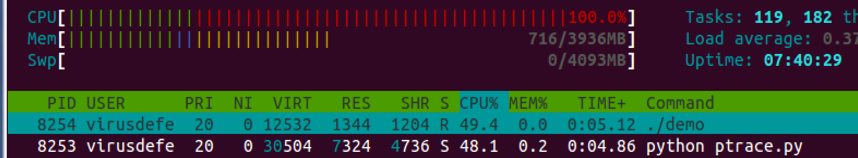
\includegraphics[width=0.9\textwidth]{ptrace-parent-process}
\caption{ptrace父进程也消耗大量CPU资源}
\end{figure}

测试环境:Ubuntu 14.04,虚拟化单核,主机MacBook Pro Intel(R) Core(TM) i5-4278U CPU @ 2.60GHz。

seccomp是一种侵入式策略,需要在代码执行之前加载,而不是ptrace那样在父进程中全部控制。开发过程中设计过几种加载seccomp的方法,但是都逐渐的发现存在绕过,最终方案是在\texttt{execve}之前加载,并且对\texttt{execve}这个本该是黑名单的系统调用进行了参数过滤,下面章节是详细的分析。

\subsubsection{动态库使用\texttt{LD\_PRELOAD}加载的绕过}

在编写代码的时候一般是从main函数开始的,但是实际进程执行的时候并不是,在main函数执行之前还有一些初始化函数,比如\texttt{start}和\texttt{\_\_libc\_start\_main}函数\cite{linux-process-start}。如果可以hook这些函数就可以在用户代码执行之前执行加载seccomp的代码了,很明显可以使用动态库来覆盖\texttt{\_\_libc\_start\_main},加载seccomp策略,然后模拟正常执行的去调用main函数,示例如下

\begin{verbatim}

typedef int (*main_t)(int, char **, char **);  
int __libc_start_main(main_t main, int argc, 
    char *__unbounded *__unbounded ubp_av,
    ElfW(auxv_t) *__unbounded auxvec,
    __typeof (main) init,
    void (*fini) (void),
    void (*rtld_fini) (void), void *__unbounded
    stack_end)
{
    int i;
    ssize_t len;
    void *libc;
    int (*libc_start_main)(main_t main,
        int,
        char *__unbounded *__unbounded,
        ElfW(auxv_t) *,
        __typeof (main),
        void (*fini) (void),
        void (*rtld_fini) (void),
        void *__unbounded stack_end);
    libc = dlopen("libc.so.6", RTLD_LOCAL  | RTLD_LAZY);
    if (!libc) {
        exit(1);
    }
  
    libc_start_main = dlsym(libc, "__libc_start_main");
    if (!libc_start_main) {
        exit(2);
}
// TODO: load seccomp rules
    return ((*libc_start_main)(main, argc, ubp_av, auxvec,
                 init, fini, rtld_fini, stack_end));
}

\end{verbatim}

上述代码由 https://github.com/quark-zju/lrun 修改而来,完整代码和编译选项可见GitHub。GitHub上另外一个项目 https://github.com/daveho/EasySandbox 也使用了类似的方法。并且EasySandbox的说明\cite{easy-sandbox-bypass}中也提到了这种实现可能的绕过:如果用户程序自定义了\\\texttt{\_\_libc\_start\_main}函数,动态库中的\texttt{\_\_libc\_start\_main}就不会执行,但是这个需要编译选项\texttt{-nostdlib}的支持,如果没有这个编译选项,就会出现编译错误。

将上述代码加载seccomp的部分删除,补充main函数,在Ubuntu 14.04上使用gcc 4.8.4进行编译并没有出现编译错误,并且执行的是确实是用户的而不是沙箱的\texttt{\_\_libc\_start\_main}函数,导致沙箱被绕过。所以这种方案只能放弃,如果没有这个问题,确实是一个很好的做法,不需要修改任何代码,只要加载一个动态库,后续的进程行为都被我们控制了。

\subsubsection{同名库函数覆盖导致的绕过}

为了避免\texttt{\_\_libc\_start\_main}函数被覆盖,可以将沙箱代码和用户代码一起编译,这样用户代码中如果也定义了\texttt{\_\_libc\_start\_main}就会导致编译错误,实际验证也是这样的。但是用户代码中也可以覆盖一些头文件中的函数为空函数,导致沙箱失效,比如\texttt{seccomp\_rule\_add}、\texttt{seccomp\_release}函数等。

\begin{verbatim}
#include <stdio.h>
#include <seccomp.h>

int seccomp_rule_add(scmp_filter_ctx ctx, uint32_t action, 
                     int syscall, unsigned int arg_cnt, ...) {
    printf("This is a fake seccomp_rule_add\n");
    return 0;
}
int seccomp_load(scmp_filter_ctx ctx) {
    return 0;
}
void seccomp_release(scmp_filter_ctx ctx) {}
int main()
{
    return 0;
}
\end{verbatim}

\texttt{gcc main.c sandbox.c -ldl -lseccomp -o user\_code \&\& ./user\_code}编译运行发现输出了This is a fake seccomp\_rule\_add。

\subsubsection{在\texttt{execve}之前加载seccomp}

在\texttt{execve}之前加载seccomp看起来是没有问题的,但是seccomp策略是白名单类型的,要这样做的话必须将\texttt{execve}也加入白名单,而这确确实实是一个危险函数,也可以直接用来执行系统命令,所以也是一个潜在的绕过,我们可以使用seccomp的参数过滤来过滤\texttt{execve}的参数,可执行文件路径只能是确定的。例如

\begin{verbatim}
#include <stdio.h>
#include <unistd.h>
#include <seccomp.h>
  
int main() {
  char file_name[30] = "/bin/ls";
  char dangerous_file_name[30] = "/bin/rm";
  char *argv[] = {"/", NULL};
  char *env[] = {NULL};
  scmp_filter_ctx ctx;
  ctx = seccomp_init(SCMP_ACT_ALLOW);
  seccomp_rule_add(ctx, SCMP_ACT_KILL, SCMP_SYS(execve), 1,
                        SCMP_A0(SCMP_CMP_NE, file_name));
  seccomp_load(ctx);
  execve(file_name, argv, env);
  return 0;
}
\end{verbatim}

如果把\texttt{file\_name}换成\texttt{dangerous\_file\_name},就会提示bad system call。这样就解决了\texttt{execve}可能带来的绕过。

\subsubsection{系统调用白名单}

确定了加载seccomp的方法之后,只需要确定哪些系统调用是安全的就可以了。在Linux系统下,使用\texttt{strace}命令可以获取进程运行所有的系统调用,在抽样分析了OJ上提交过的代码之后,得到了以下系统调用白名单。
\begin{table}[H]
\centering
\caption{系统调用白名单}
\begin{tabular}{ |c|c| } 
\hline
系统调用 & 说明 \\
\hline
open &打开一个文件 \\
\hline
read &读取文件 \\
\hline
write &写文件 \\
\hline
close &关闭文件 \\
\hline
fstat &检测文件状态 \\
\hline
mmap &\multirow{5}{4em}{内存分配相关} \\ 
munmap& \\ 
mprotect& \\ 
arch\_ptctl& \\
brk& \\
\hline
access &检查文件权限 \\
\hline
exit\_group &结束进程的所有线程 \\
\hline
\end{tabular}
\end{table}
和\texttt{execve}一样,\texttt{write}系统调用也需要过滤参数。当\texttt{write}的参数为1和2的时候,代表\texttt{stdout}和\texttt{strerr},其余的参数值代表某个文件的文件描述符,如果不限制\texttt{write}的参数,进程就可以写任意文件了。

使用了下面的代码实现

\begin{verbatim}
// only fd 0 1 2 are allowed
if (seccomp_rule_add(ctx, SCMP_ACT_ALLOW, SCMP_SYS(write), 1, 
                          SCMP_A0(SCMP_CMP_LE, 2))) {
    LOG_FATAL("load dup2 rule failed");
    ERROR(LOAD_SECCOMP_FAILED);
}
\end{verbatim}

\subsubsection{用户权限控制}

Linux上用户分为root用户和非root用户。root用户拥有最高权限,而nobody用户权限非常低,可以使用nobody用户来运行风险级别比较高的进程,比如各种Web服务器软件。沙箱也使用了这个用户来运行用户的代码,一旦沙箱机制被攻破,还可以通过Linux用户权限控制避免更大的危害。
Linux中提供了\texttt{setuid}函数,可以以uid用户身份运行,但是需要root权限来调用。

使用了下面的代码实现

\begin{verbatim}
if (setgid(NOBODY_GID)) {
    LOG_FATAL("setgid failed, errno: %d", errno);
    ERROR(SET_GID_FAILED);
}
if (setuid(NOBODY_UID)) {
    LOG_FATAL("setuid failed, errno: %d", errno);
    ERROR(SET_UID_FAILED);
}
\end{verbatim}

\subsubsection{编译器安全}

这是一个容易被忽视的方面,目前已知的主要有以下几种。

一是引用某些可以无限输出的文件,比如\texttt{\#include</dev/random>},编译器会一直读取,导致卡死。

二是让编译器产生大量的错误信息,比如下面一段代码,可以让g++编译器产生数G的错误日志。

\begin{verbatim}
int main()
{
    struct x struct z<x(x(x(x(x(x(x(x(x(x(x(x(x(x(x(y,x(y><y*,x(y*w>v<y*,w,x{}
    return 0;
}
\end{verbatim}

处理方法就是编译器运行的时候也要控制CPU时间和实际运行时间,同时使用编译器参数\texttt{-fmax-errors=N}来控制最大错误数量。

三是\texttt{C++}的模板元编程,部分代码是编译期执行的,可以构造出让编译器产生大量计算的代码。

和第二个问题一样,实际大量的去占用资源的并不是编译器进程,而是编译器的子进程,在单纯使用\texttt{setitimer}方法的时候并无法控制子进程,所以还需要\texttt{setrlimit}的辅助。

四是引用一些敏感文件可能导致信息泄露,比如\texttt{\#include</etc/shadow/>},会在编译错误的信息中泄露文件开头的内容。

\subsubsection{小结}
我们主要是从系统调用的层面来保证安全性的,而Linux还有很多其他的特性可以用来保证安全,比如\texttt{chroot}、\texttt{cgroups}、\texttt{user\_namespace}等。还可以将代码放入Docker或者虚拟机中运行,使用Docker或者虚拟机的隔离性进一步提高安全性。

在开发过程中还遇到了很多细节问题,如不同操作系统系统调用的不同,多线程竞态条件的问题等等。实现一个安全的判题沙箱是很困难的,需要对Linux API有深入的了解,有时还需要找源码或者反汇编查看一些底层的实现。

\clearpage
\section{系统测试与部署}

\subsection{使用持续集成构建代码与测试环境}

在系统开发过程中,为了保证代码质量,编写了大量的单元测试,核心模块测试覆盖率接近100\%, 并使用了travis-ci构建集成测试,流程如下:

\begin{itemize}
    \item[-] 绑定Github和travis-ci项目,项目中创建相关的配置文件。
    \item[-] 每次向Github push代码或者发起新的Merge Request的时候,Github都会向travis-ci发送一个消息,这样travis-ci就可以拉取代码进行集成测试了。
    \item[-] 测试成功或者失败会向邮箱发送邮件,便于了解最新的状态。
\end{itemize}

\begin{figure}[H]
\centering
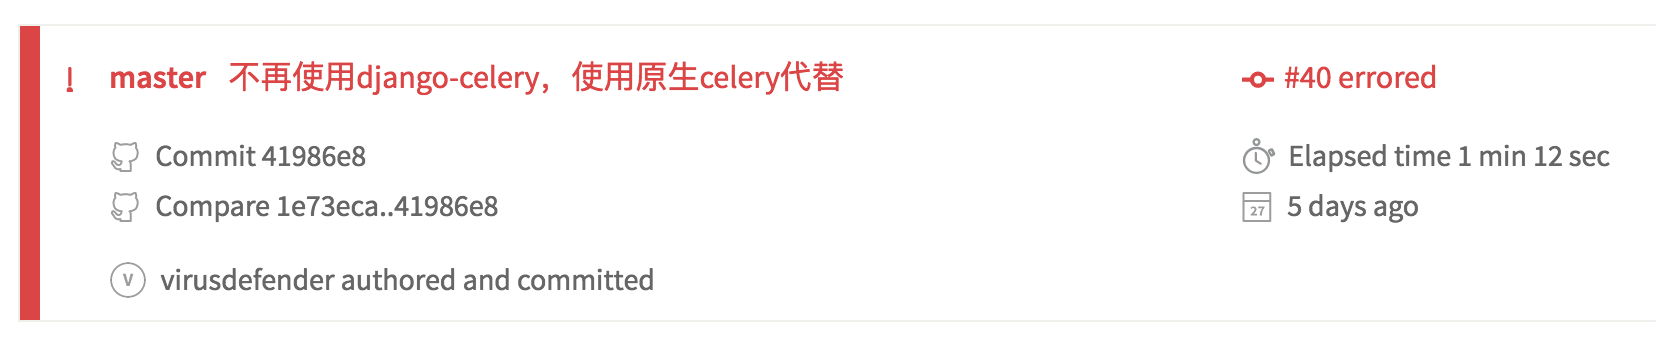
\includegraphics[width=0.9\textwidth]{ci-failed}
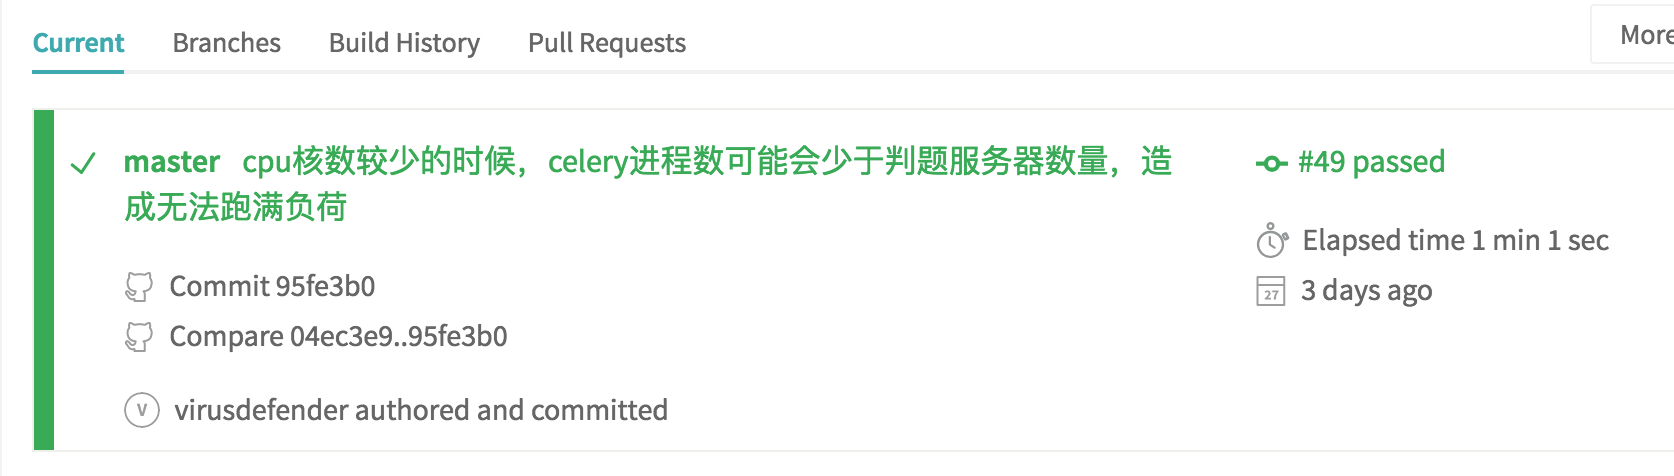
\includegraphics[width=0.9\textwidth]{ci-succeeded}
\caption{CI测试失败和通过的界面}
\end{figure}

如果测试通过,自动化部署的机器人就会拉取最新的代码,通过实现设定的脚本,自动化的更新测试环境,包括构建新的Docker镜像、应用数据库修改和重启Web Server等。

\subsection{使用Docker简化部署难度}
Docker是革命性的产品,通过镜像和容器大大简化了互联网产品的测试与部署难度。

本系统只需要通过Dockerfile全自动构建Docker镜像,然后简单配置docker-compose.yml文件,包括目录映射、部分环境变量和端口映射等,就可以直接运行。相比传统部署方式,隔离了服务器环境与系统的运行环境,大大降低了部署难度。

\texttt{Dockerfile}文件示例
\begin{verbatim}
FROM python:2.7
ENV PYTHONBUFFERED 1
RUN mkdir -p /code/log /code/test_case /code/upload
WORKDIR /code
ADD requirements.txt /code/
RUN pip install -r requirements.txt && rm /etc/apt/sources.list
ADD sources.list /etc/apt/
RUN curl -sL https://deb.nodesource.com/setup | bash -
RUN apt-get -y install nodejs
ADD gunicorn.conf /etc
ADD supervisord.conf /etc
ADD task_queue.conf /etc
EXPOSE 8080
CMD bash /code/dockerfiles/oj_web_server/run.sh
\end{verbatim}

\begin{figure}[H]
\centering
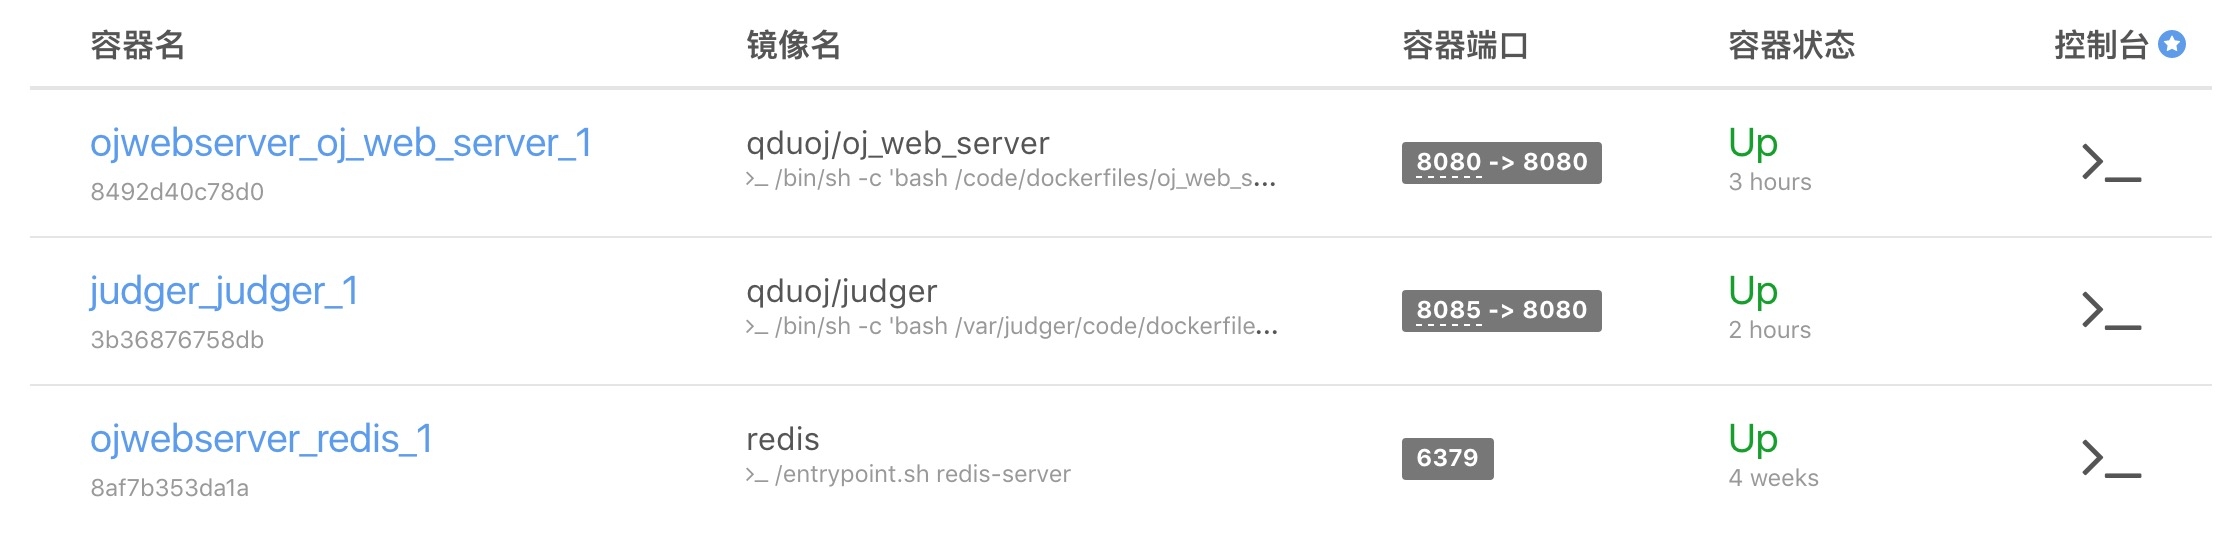
\includegraphics[width=\textwidth]{oj-docker}
\caption{OJ Docker运行情况}
\end{figure}

\begin{center}
\title{谢~~辞}
\date{}
\maketitle
\end{center}

时光荏苒,岁月如梭,写下这篇致谢的时候,大学生活就要接近尾声了。还能在青大有最后一个多月的时光,虽有激动,但心中更多的是不舍。

感谢信息工程学院(现计算机学院科学技术学院)创新实验室的李建波老师和青大ACM队的杜祥军老师,在创新实验室和ACM队的近三年时间,是我快速成长的三年,同时实验室的同学们也给予了非常多的帮助,让我能一直坚定的走下去,真的很高兴遇到大家。

感谢参与部分模块开发和改进孙小文、王涛、孙晓冬和江学磊同学,感谢给该毕业设计提出过问题和建议的朋友们。

感谢指导老师陈宇,在本论文的写作过程中提出了非常多的建设性意见。



\clearpage
\renewcommand{\refname}{参考文献}
\printbibliography
\afterpage{\blankpage}
\end{document}